\documentclass[oneside]{book}
\usepackage{zxjatype}

\setjamainfont[BoldFont=IPAゴシック]{IPA明朝}
\setjasansfont{IPAゴシック}
\setjamonofont{IPAゴシック}
\usepackage{unicode-math}

% New line height: 1.05 * 1.2 = 1.26
\renewcommand{\baselinestretch}{1.05}

\usepackage{polyglossia}

% To be able to use '\-/' in place of '-' inside \code{}
% so that long function names containing hyphens 
% can be broken up after the hyphen:
\usepackage[shortcuts]{extdash} 

% So that file names with multiple dots don't confuse 
% graphicx package when using \includegraphics command:
\usepackage[multidot]{grffile}
\usepackage{graphicx}

\usepackage[usenames,dvipsnames,x11names]{xcolor}
\usepackage{amsmath}

% To use Libertine letters and numbers,
% but tx-style operators in math environment:
\usepackage[libertine]{newtxmath} 

% Workaround to fix mismatched left and right math delimiters. Taken from: 
% http://tex.stackexchange.com/questions/63410/parentheses-differ-xelatex-fontspec-newtxmath-libertine
\DeclareSymbolFont{parenthesis}{T1}{fxl}{m}{n}
\DeclareMathDelimiter{(}{\mathopen}{parenthesis}{"28}{largesymbols}{"00}
\DeclareMathDelimiter{)}{\mathclose}{parenthesis}{"29}{largesymbols}{"01}
\DeclareMathDelimiter{[}{\mathopen}{parenthesis}{"5B}{largesymbols}{"02} 
\DeclareMathDelimiter{]}{\mathclose}{parenthesis}{"5D}{largesymbols}{"03} 
\DeclareMathDelimiter{\lbrace}{\mathopen}{parenthesis}{"7B}{largesymbols}{"08} 
\DeclareMathDelimiter{\rbrace}{\mathclose}{parenthesis}{"7D}{largesymbols}{"09}

\usepackage{fancyvrb}
\usepackage{imakeidx}
\usepackage[totoc,font=footnotesize]{idxlayout}
\usepackage{fancyhdr}
\pagestyle{plain}
\usepackage[final]{pdfpages} % inserts pages from a pdf file

% Page geometry for 10-inch tablets:
\usepackage[papersize={148mm,197mm},
            top=21mm,
            textwidth=111mm,
            textheight=148mm,
            hcentering,
]{geometry}

\usepackage{titlesec}  % to change the appearance of section titles 
\usepackage{listings}  % for syntax highlighted code listings
\usepackage{verbatim}  % for simple verbatim and comment environments
\usepackage{enumerate} % allows customized labels in enumerations
\usepackage{hyperref}  % makes cross references and URLs clickable 
\definecolor{LinkRed}{HTML}{80171F}
\hypersetup{
  pdfauthor={Harold Abelson, Gerald Jay Sussman, Julie Sussman},
  pdftitle={Structure and Interpretation of Computer Programs, 2nd ed.},
  pdfsubject={computer science, programming, abstraction},
  colorlinks=true,
  linkcolor=LinkRed,
  urlcolor=LinkRed,
}

% Document colors 
\definecolor{SchemeLight}  {HTML} {686868}
\definecolor{SchemeSteel}  {HTML} {787878}
\definecolor{SchemeDark}   {HTML} {262626}
\definecolor{SchemeBlue}   {HTML} {4172A3}
\definecolor{SchemeGreen}  {HTML} {487818}
\definecolor{SchemeBrown}  {HTML} {A07040}
\definecolor{SchemeRed}    {HTML} {AD4D3A}
\definecolor{SchemeViolet} {HTML} {7040A0}
\definecolor{DropCapGray}  {HTML} {A8A8A8}
\definecolor{ChapterGray}  {HTML} {C8C8C8}

\usepackage{lettrine}  % adds commands that make drop capitals
\renewcommand{\LettrineFontHook}{\rmfamily\bfseries\color{DropCapGray}}
\renewcommand{\DefaultLraise}{0.00}
\renewcommand{\DefaultLoversize}{0.02}
\renewcommand{\DefaultLhang}{0.12}
\setlength{\DefaultFindent}{1pt}
\setlength{\DefaultNindent}{0em}

\lstset{%
  % Scheme syntax highlighter
    columns=fixed,
    extendedchars=true,
    upquote=true,
    showstringspaces=false,
    sensitive=false,
    mathescape=true,
    escapechar=~,
    alsodigit={>,<,/,-,=,!,?,*},
    alsoletter=',
    morestring=[b]",
    morecomment=[l];,
    % Keyword list taken form functional.py in Pygments package:
    morekeywords={lambda, define, if, else, cond, and, or, case,%
      let, let*, letrec, begin, do, delay, set!, =>, quote,%
      quasiquote, unquote, unquote-splicing, define-syntax, let-syntax,%
      letrec-syntax, syntax-rules},
    % If keywords are quoted, they must not be highlighted:
    emph={'lambda, 'define, 'if, 'else, 'cond, 'and, 'or, 'case,%
      'let, 'let*, 'letrec, 'begin, 'do, 'delay, 'set!, '=>, 'quote,%
      'quasiquote, 'unquote, 'unquote-splicing, 'define-syntax, 'let-syntax,%
      'letrec-syntax, 'syntax-rules}, 
    emphstyle=\color{SchemeDark},
    % Paint error red:
    emph={[2]error},emphstyle=[2]\color{SchemeRed},%
    % Builtins taken from functional.py:
    emph={[3]*, +, -, /, <, <=, =, >, >=, abs, acos, angle,
        append, apply, asin, assoc, assq, assv, atan,
        boolean?, caaaar, caaadr, caaar, caadar, caaddr, caadr,
        caar, cadaar, cadadr, cadar, caddar, cadddr, caddr,
        cadr, call-with-current-continuation, call-with-input-file,
        call-with-output-file, call-with-values, call/cc, car,
        cdaaar, cdaadr, cdaar, cdadar, cdaddr, cdadr, cdar,
        cddaar, cddadr, cddar, cdddar, cddddr, cdddr, cddr,
        cdr, ceiling, char->integer, char-alphabetic?, char-ci<=?,
        char-ci<?, char-ci=?, char-ci>=?, char-ci>?, char-downcase,
        char-lower-case?, char-numeric?, char-ready?, char-upcase,
        char-upper-case?, char-whitespace?, char<=?, char<?, char=?,
        char>=?, char>?, char?, close-input-port, close-output-port,
        complex?, cons, cos, current-input-port, current-output-port,
        denominator, display, dynamic-wind, eof-object?, eq?,
        equal?, eqv?, eval, even?, exact->inexact, exact?, exp,
        expt, floor, for-each, force, gcd, imag-part,
        inexact->exact, inexact?, input-port?, integer->char,
        integer?, interaction-environment, lcm, length, list,
        list->string, list->vector, list-ref, list-tail, list?,
        load, log, magnitude, make-polar, make-rectangular,
        make-string, make-vector, map, max, member, memq, memv,
        min, modulo, negative?, newline, not, null-environment,
        null?, number->string, number?, numerator, odd?,
        open-input-file, open-output-file, output-port?, pair?,
        peek-char, port?, positive?, procedure?, quotient,
        rational?, rationalize, read, read-char, real-part, real?,
        remainder, reverse, round, scheme-report-environment,
        set-car!, set-cdr!, sin, sqrt, string, string->list,
        string->number, string->symbol, string-append, string-ci<=?,
        string-ci<?, string-ci=?, string-ci>=?, string-ci>?,
        string-copy, string-fill!, string-length, string-ref,
        string-set!, string<=?, string<?, string=?, string>=?,
        string>?, string?, substring, symbol->string, symbol?,
        tan, transcript-off, transcript-on, truncate, values,
        vector, vector->list, vector-fill!, vector-length,
        vector-ref, vector-set!, vector?, with-input-from-file,
        with-output-to-file, write, write-char, zero?},
    emphstyle=[3]\color{SchemeViolet},%
    %
    basicstyle=\color{SchemeLight}\ttfamily,
    keywordstyle=\color{SchemeBlue}\bfseries,
    identifierstyle=\color{SchemeDark},
    stringstyle=\color{SchemeGreen},
    commentstyle=\color{SchemeLight}\itshape,
}
  
\newcommand{\acronym}[1]{\textsc{\MakeLowercase{#1}}}
\newcommand{\newterm}[1]{\index{#1}\emph{#1}}
\newcommand{\strong}[1]{\textbf{#1}}
\newcommand{\var}[1]{\textsl{#1}}
\newcommand{\code}[1]{\texttt{#1}}
\newcommand{\link}[1]{\hyperref[#1]{#1}}
\newcommand{\heading}[1]{{\sffamily\bfseries #1}}
\newcommand{\dark}{\color{SchemeDark}}

\newenvironment{example}%
  {\verbatim\small}%
  {\endverbatim}

\newenvironment{smallexample}%
  {\verbatim\footnotesize}%
  {\endverbatim}

\lstnewenvironment{scheme}[1][]
{\lstset{basicstyle=\ttfamily\small\color{SchemeLight},#1}}
{}

\lstnewenvironment{smallscheme}[1][]
{\lstset{basicstyle=\ttfamily\footnotesize\color{SchemeLight},#1}}
{}

\titleformat{\chapter}[display]
  {\color{SchemeDark}\normalfont\sffamily\bfseries\LARGE}
  {\filright \color{ChapterGray}\fontsize{3em}{0em}\selectfont
    \oldstylenums{\thechapter}}
  {1em}
  {\filright}
  
\titleformat{\section}
{\color{SchemeDark}\normalfont\Large\sffamily\bfseries}
{\color{SchemeSteel}\thesection}{0.8em}{}

\titleformat{\subsection}
{\color{SchemeDark}\normalfont\large\sffamily\bfseries}
{\color{SchemeSteel}\thesubsection}{0.8em}{}

\titleformat{\subsubsection}
{\color{black}\normalfont\normalsize\sffamily\bfseries}
{\color{SchemeSteel}\thesubsubsection}{0.8em}{}

\setcounter{secnumdepth}{3}
\setcounter{tocdepth}{3}

\frenchspacing
\makeindex

%====================%
%  End of preamble.  %
%====================%

\begin{document}
\pagenumbering{roman}
\VerbatimFootnotes

%             **********************************************************
%         sicp
%            Structure and Interpretation of Computer Programs, 2e
%             Unofficial Texinfo Format
%
% utfversion      2.andresraba5.2 
% utfversiondate  February 10, 2014
%
%             This file is licensed under a Creative Commons 
%             Attribution-ShareAlike 3.0 Unported License 
%             http://creativecommons.org/licenses/by-sa/3.0/
%             
%             This is a Texinfo file.  To convert it to Info hypertext
%             format, you will need the `makeinfo' program from the GNU
%             Texinfo package.  To produce a PDF, use `texi2pdf'. 
%             For more information about this file,
%             see the text under `\label{UTF' below.}
%             
%             Various versions of sicp.texi and preformatted sicp.info
%             can be found at the following Web pages:
%             
%                 http://www.neilvandyke.org/sicp-texi/
%                 http://sicpebook.wordpress.com/
%                 [add your own here]
%             
%             **********************************************************

% HISTORY:
%
% * Version 1 (April, 2001) by Lytha Ayth.
%
% * Version 2 (April 20, 2001) by Lytha Ayth.
%
% * Version 2.nwv1 (March 11, 2002) by Neil W. Van Dyke.
%   Cosmetic change to heading in Info format, and comment changes.
% 
% * Version 2.neilvandyke1 (February 10, 2003) by Neil W. Van Dyke
%   Correction to Exercise 1.39 formula, spotted by Steve VanDevender.
%   Added URL of Abelson and Sussman video lectures.
%
% * Version 2.neilvandyke2 (unreleased)
%
% * Version 2.neilvandyke3 (April 20, 2006) by Neil W. Van Dyke
%   Pedro Kr\"oger patch to add missing Lisp example.
%
% * Version 2.neilvandyke4 (January 10, 2007) by Neil W. Van Dyke
%   Brad Walker patch to add \code{@dircategory} and \code{@direntry}.
%
% * Version 2.andresraba1 (May 23, 2011) by Andres Raba.
%   Mathematics typeset in TeX, figures redrawn in vector graphics,
%   typeface changed, cross-references improved, hyperlinks added,
%   known errors and typos corrected.
%
% * Version 2.andresraba2 (November 21, 2011) by Andres Raba.
%   Minor change to the appearance of diagrams. Adjusted page layout.
%   Fixed some typos. License changed from CC BY-NC to CC BY-SA.
%
% * Version 2.andresraba3 (November 22, 2012) by Andres Raba.
%   Improved layout and pagination. Included list of figures.
%   Added punctuation to displayed math. Updated citation links.

% * (Version 2.andresraba4 is a pocket version, described in
%   sicp-pocket.texi.)

% * Version 2.andresraba5 (September 20, 2013) by Andres Raba.
%   Texinfo source is converted to LaTeX. Pages are redesigned.

% The Algorithmic Language Scheme

\frontmatter

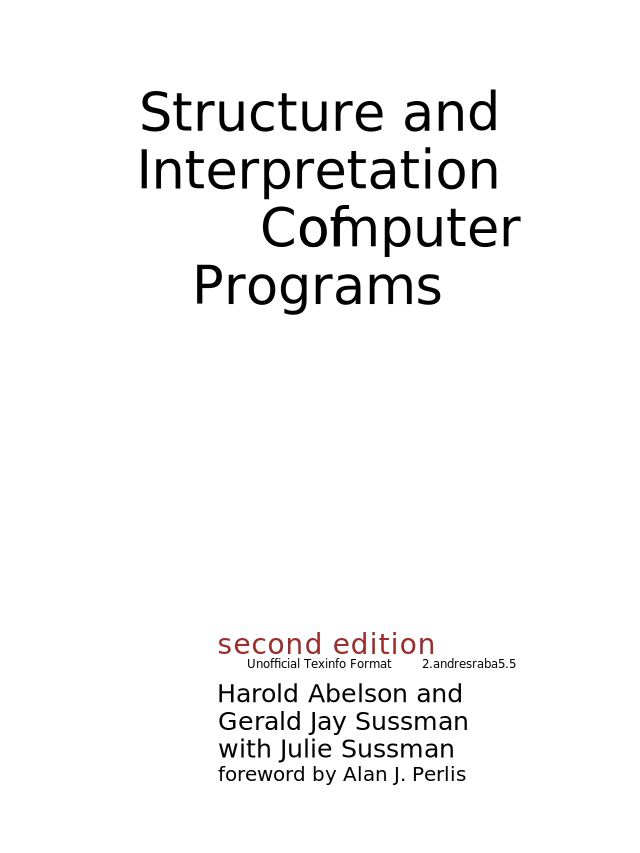
\includepdf[scale=0.92]{coverpage.pdf}

\pagebreak

\vspace*{\fill}
\thispagestyle{empty}

\begin{small}

\noindent
{\copyright}1996 by The Massachusetts Institute of Technology

\vspace{1.26em}
\noindent
Structure and Interpretation of Computer Programs,\\
second edition

\vspace{1.26em}
\noindent
Harold Abelson and Gerald Jay Sussman\\
with Julie Sussman, foreword by Alan J. Perlis

\vspace{1.6em}
\noindent
\includegraphics[width=3mm]{fig/icons/cc.pdf}
\includegraphics[width=3mm]{fig/icons/by.pdf}
\includegraphics[width=3mm]{fig/icons/sa.pdf}

\vspace{0.4em}
\noindent
This work is licensed under a Creative Commons\\ 
Attribution-ShareAlike 3.0 Unported License\\
(\href{http://creativecommons.org/licenses/by-sa/3.0/}{\acronym{CC BY-SA} 3.0}).
Based on a work at \href{http://mitpress.mit.edu/sicp/}{mitpress.mit.edu}.

\vspace{1.26em}
\noindent
The \acronym{MIT} Press\\
Cambridge, Massachusetts\\ 
London, England

\vspace{1.26em}
\noindent
McGraw-Hill Book Company\\
New York, St. Louis, San Francisco,\\ 
Montreal, Toronto

\vspace{1.26em}
\noindent
Unofficial Texinfo Format \href{http://sicpebook.wordpress.com}{2.andresraba5.2} (February 10, 2014),\\ 
based on \href{http://www.neilvandyke.org/sicp-texi/}{2.neilvandyke4} (January 10, 2007).

\vspace{1.26em}
\noindent
日本語: by \href{http://d.hatena.ne.jp/minghai/}{minghai} based on 2.andresraba5.2 (March 31, 2014).

\end{small}

\pagebreak

\tableofcontents

\small  % Added by minghai. (Japanese fonts looks too big.)

%=======================================================================================================

\label{UTF}
\chapter*{Unofficial Texinfo Format}
\addcontentsline{toc}{chapter}{Unofficial Texinfo Format}

This is the second edition \acronym{SICP} book, from Unofficial Texinfo
Format.

これは\acronym{SICP}の第二版非公式Texinfo版です。

You are probably reading it in an Info hypertext browser, such as the Info
mode of Emacs.  You might alternatively be reading it {\TeX}-formatted on your
screen or printer, though that would be silly.  And, if printed, expensive.

あなたは恐らくこれをEmacsのInfoモードの様なハイパーテキストブラウザで読んで
いることでしょう。他にも{\TeX}で組版した物を画面や印刷して読んでいるかもしれませんが
それはバカバカしい上に高くつきます。

The freely-distributed official \acronym{HTML}-and-\acronym{GIF} format was
first converted personally to Unofficial Texinfo Format (\acronym{UTF})
version 1 by Lytha Ayth during a long Emacs lovefest weekend in April, 2001.

公式に無料で公開された\acronym{HTML}-and-\acronym{GIF}版を
Lytha Aythが最初に私的に、2001年4月の長いEmacs Lovefest Weekendの間に
非公式Texinfo版(\acronym{UTF})バージョン1へと変換しました。

The \acronym{UTF} is easier to search than the \acronym{HTML} format.  It is
also much more accessible to people running on modest computers, such as
donated '386-based PCs.  A 386 can, in theory, run Linux, Emacs, and a Scheme
interpreter simultaneously, but most 386s probably can't also run both Netscape
and the necessary X Window System without prematurely introducing budding young
underfunded hackers to the concept of \newterm{thrashing}.  UTF can also fit
uncompressed on a 1.44\acronym{MB} floppy diskette, which may come in handy for
installing UTF on PCs that do not have Internet or LAN access.

\acronym{UTF}はHTML版よりも検索がより簡単です。また寄付された古い386の様な
質素な計算機上で行う人々にとってよりアクセスが容易です。386は理論的にはLinux、Emacs、
Schemeインタプリタを同時に実行できます。しかし多くの386は恐らくNetscapeと必要なX Window
Systemを事前に芽の出かけた資金不足の若いハッカーに\newterm{thrashing}(スラッシング)の
概念を教えることなしに動かすことはできないでしょう。UTFはまた圧縮無しでも1.44\acronym{MB}
のフロッピーディスケットに収まります。これはインターネットやLANへの接続環境の無いPC
にインストールする場合に役立つでしょう。

The Texinfo conversion has been a straight transliteration, to the extent
possible.  Like the {\TeX}-to-\acronym{HTML} conversion, this was not without
some introduction of breakage.  In the case of Unofficial Texinfo Format,
figures have suffered an amateurish resurrection of the lost art of
\acronym{ASCII}.  Also, it's quite possible that some errors of ambiguity
were introduced during the conversion of some of the copious superscripts (`\^{}')
and subscripts (`\_').  Divining \emph{which} has been left as an exercise to
the reader. But at least we don't put our brave astronauts at risk by encoding
the \emph{greater-than-or-equal} symbol as \code{<u>\&gt;</u>}.

Texinfoへの変換は可能な範囲で直接的な翻字でした。{\TeX}-to-\acronym{HTML}変換の様に
ある程度の破れが含まれること無しにはできませんでした。非公式TexInfo形式においては
図が「失なわれた技術」であるアスキーアートによる下手糞な"復活"を被りました。また
多量の上付き文字と下付き文字のいくつかの変換の間に不明瞭さによる変換の
失敗が含まれてしまった可能性が大いにあります。読者への課題として残されたと予測します。
しかし、最低でも\emph{``以上''}の記号を\texttt{<u>\&gt;</u>}と符号化することで
我等の勇敢な宇宙飛行士を危険に置くようなことはしませんでした。

If you modify \texttt{sicp.texi} to correct errors or improve the
\acronym{ASCII} art, then update the \code{hoge}
line to reflect your delta.  For example, if you started with Lytha's version
\code{1}, and your name is Bob, then you could name your successive versions
\code{1.bob1}, \code{1.bob2},  \dots , \code{1.bob\textit{n}}. 

もしあなたが\texttt{sicp.texi}を変更しエラーを訂正したり、アスキーアートを向上させたなら
\code{@set utfversion {utfversion}}の行を更新し、あなたの修正を反映して下さい。
例えば、もしあなたがLythaのバージョン\code{1}で開始し、あなたの名前がBobなら、改訂版は
\code{1.bob1}, \code{1.bob2}, \dots , \code{1.bob\textit{n}}です。また\code{utfversiondate}も更新
して下さい。もしあなたが自分の改訂版をWeb上で配布したいのなら文字列``sicp.texi''を
ファイルやWebページのどこかに埋め込んでおけば人々にとってWeb検索エンジンから
探すことが簡単になるでしょう。

It is believed that the Unofficial Texinfo Format is in keeping with the
spirit of the graciously freely-distributed \acronym{HTML} version.  But you
never know when someone's armada of lawyers might need something to do, and get
their shorts all in a knot over some benign little thing, so think twice before
you use your full name or distribute Info, \acronym{DVI}, PostScript, or
\acronym{PDF} formats that might embed your account or machine name.

非公式Texinfo形式は寛大にも自由の下に配布された\acronym{HTML}版の魂を引き継いで
いると信じられています。しかし、いつ誰かの法律家の大艦隊が良心に基づく小さな事に対して非常に腹を立て
何かを行わなければならなくなるかもしれません。ですのであなたのフルネームを
使ったり、あなたのアカウントやマシン名を含むInfo, \acronym{DVI}, PostScript, \acronym{PDF}形式
を配布する前に良く良く考えて下さい。

\noindent
\textit{Peath, Lytha Ayth}

\vspace{1.0em}
\noindent
\textbf{Addendum:} See also the \acronym{SICP} video lectures by Abelson and Sussman:\\
at \href{http://groups.csail.mit.edu/mac/classes/6.001/abelson-sussman-lectures/}{\acronym{MIT CSAIL}} or 
\href{http://ocw.mit.edu/courses/electrical-engineering-and-computer-science/6-001-structure-and-interpretation-of-computer-programs-spring-2005/video-lectures/}{\acronym{MIT OCW}}.

\textbf{付録:}AbelsonとSussmanによる\acronym{SICP}のビデオレクチャーもご覧下さい。\\
\href{http://groups.csail.mit.edu/mac/classes/6.001/abelson-sussman-lectures/}{\acronym{MIT CSAIL}}
\href{http://ocw.mit.edu/courses/electrical-engineering-and-computer-science/6-001-structure-and-interpretation-of-computer-programs-spring-2005/video-lectures/}{\acronym{MIT OCW}}.


\vspace{0.5em}
\noindent 
\textbf{Second Addendum:} Above is the original introduction to the \acronym{UTF} 
from 2001. Ten years later, \acronym{UTF} has been transformed: mathematical 
symbols and formulas are properly typeset, and figures drawn in 
vector graphics. The original text formulas and \acronym{ASCII} art figures 
are still there in the Texinfo source, but will display only when compiled 
to Info output. At the dawn of e-book readers and tablets, reading a 
\acronym{PDF} on screen is officially not silly anymore. Enjoy!

\noindent
\textbf{付録2:} 上記は2001年の元の\acronym{UTF}の紹介です。
10年後、\acronym{UTF}は一変しました。数学上の記号と式は適切に組版され、図は
ベクターグラフィックにより描かれています。元のテキスト形式とアスキーアートの図
は今でもTexinfoのソースに残っていますが、Info形式でコンパイルした場合のみ
表示されます。電子書籍リーダーとタブレットの夜明けに画面上で\acronym{PDF}を
読むことは正式に、最早バカバカしいことでは無くなりました。楽しんで下さい!

\vspace{0.5em}
\noindent
\textit{A.R, May, 2011}

%============================================================================================================

\label{Dedication}
\chapter*{Dedication}
\addcontentsline{toc}{chapter}{Dedication}

\lettrine{T}{his book is dedicated}, in respect and admiration, to the spirit that lives in
the computer.

この本を、尊敬と賛美を込めて、コンピュータの中に住む妖精に捧げます。

\begin{quote}
``I think that it's extraordinarily important that we in computer science keep
fun in computing.  When it started out, it was an awful lot of fun. Of course,
the paying customers got shafted every now and then, and after a while we began
to take their complaints seriously.  We began to feel as if we really were
responsible for the successful, error-free perfect use of these machines. 
I don't think we are.  I think we're responsible for stretching them, setting
them off in new directions, and keeping fun in the house.  I hope the field of
computer science never loses its sense of fun.  Above all, I hope we don't
become missionaries.  Don't feel as if you're Bible salesmen.   The world has
too many of those already.  What you know about computing other people will
learn. Don't feel as if the key to successful computing is only in your hands.
What's in your hands, I think and hope, is intelligence: the ability to see the
machine as more than when you were first led up to it, that you can make it
more.''

``コンピュータサイエンスに関わる私達にとってコンピュータを使用することを
楽しむことはとても大事だと私は考えます。コンピュータサイエンスが始まった時、それは
とても多くの楽しみに溢れていました。
ご存知のとおり、お金を払うお客様達は時折酷く騙されました。そして暫くして私達は
彼らの不満を真面目に受け取り始めてしまいました。
私達は考え始めてしまったのです。成功裏に、障害の無い完全なコンピュータの使用法に
ついて私達に責任があるのではないかと。
私はそうは思いません。
私は、私達がコンピュータサイエンスを伸展し、新しい方向に向かわせ、
そして仲間達と共に楽しむことに責任があると考えます。
私はコンピュータサイエンスの現場が楽しむことの感覚を失わないことを望みます。
さらに、我々が伝道師になることは望みません。
自分が聖書のセールスマンだとは思わないで下さい。
世界には既にそのような人が溢れています。
あなたが他の人々が学ぶコンピュータ利用法について何を知っているでしょう。
コンピュータ利用に成功する鍵があなたの手の中にのみあるとは決っして思わないで
下さい。
 私が思うに、そして期待することは、あなたの手の中にあるものは知性です。
それはあなたが初めて計算機に出会った時よりもより多くのことを知ることができる
能力であり、それはより多くのことを生むことができるのです。''

\noindent
---Alan J. Perlis (April 1, 1922 -- February 7, 1990)
\end{quote}

%===========================================================================================================

\label{Foreword}
\chapter*{Foreword}
\addcontentsline{toc}{chapter}{Foreword}

\vspace{-0.6em}

Educators, generals, dieticians, psychologists, and parents program.  Armies,
students, and some societies are programmed.  An assault on large problems
employs a succession of programs, most of which spring into existence en route.
These programs are rife with issues that appear to be particular to the problem
at hand.  To appreciate programming as an intellectual activity in its own
right you must turn to computer programming; you must read and write computer
programs---many of them.  It doesn't matter much what the programs are about or
what applications they serve.  What does matter is how well they perform and
how smoothly they fit with other programs in the creation of still greater
programs.  The programmer must seek both perfection of part and adequacy of
collection.  In this book the use of ``program'' is focused on the creation,
execution, and study of programs written in a dialect of Lisp for execution on
a digital computer.  Using Lisp we restrict or limit not what we may program,
but only the notation for our program descriptions.

教育者、将軍、栄養士、精神分析医、そして両親はプログラムします。軍隊、学生、そして
いくつかの社会はプログラムされます。大きな問題に対する解決は一連のプログラムを
利用します。それらのほとんどは途中でひょっこり表れます。これらのプログラムは手近な
問題に特化されて現れる成果に溢れています。プログラミングを独立した知的な活動として
理解するためにはあなたはコンピュータプログラミングに向かわねばなりません。
コンピュータプログラムを読み、書かねばなりません。それも数多くです。そのプログラムが何に
ついてであるか、またはどのような適用を担うのかは多くは関係ありません。
重要なことはそれらがどのように実行され、どれだけ滑らかに他のプログラムに対してより
大きなプログラムの作成のために適合するのかです。プログラマは部分の完全性と集合の
妥当性の両方を追求せねばなりません。この本では``プログラム''の使用はデジタル計算機上にて
実行されるためのLispの方言で書かれたプログラムの創造、実行、それに学習に焦点を当てて
います。Lispの使用はプログラム記述の表記法のみを制約、制限し、私達が何をプログラムするか
については影響を与えません。

Our traffic with the subject matter of this book involves us with three foci of
phenomena: the human mind, collections of computer programs, and the computer.
Every computer program is a model, hatched in the mind, of a real or mental
process.  These processes, arising from human experience and thought, are huge
in number, intricate in detail, and at any time only partially understood.
They are modeled to our permanent satisfaction rarely by our computer programs.
Thus even though our programs are carefully handcrafted discrete collections of
symbols, mosaics of interlocking functions, they continually evolve: we change
them as our perception of the model deepens, enlarges, generalizes until the
model ultimately attains a metastable place within still another model with
which we struggle.  The source of the exhilaration associated with computer
programming is the continual unfolding within the mind and on the computer of
mechanisms expressed as programs and the explosion of perception they generate.
If art interprets our dreams, the computer executes them in the guise of
programs!

この本の主題は3つの事象に焦点を当てます。人の心、コンピュータプログラムの集合、そして
コンピュータです。全てのコンピュータプログラムは人の心の中で生まれる現実の、または
精神的な過程のモデルです。これらの過程は人の経験と思考から浮かび上がり、数はとても
多く、詳細は入り組んで、いつでも部分的にしか理解されません。それらはコンピュータ
プログラムにより稀にしか永遠の充足としてモデル化されることはありません。従って、
例え私達のプログラムが注意深く手作りされた別個の記号の集合だとしても、連動する機能の
寄せ集めだとしても、それらは絶えず発展します。私達のモデルの知覚がより深まるにつれ、
増えるにつれ、一般化されるにつれ、モデルが究極的に準安定な位置に逹っするまで変更を
行い、その中には依然として私達が格闘するモデルが存在します。コンピュータプログラミングに
関連する歓喜の源はプログラムとして表現された仕組みの心の中とコンピュータ上で絶え間無く
続く発展であり、それにより生まれる知力の爆発です。もし技巧が私達の夢を解釈するならば、
コンピュータはプログラムとして現わされるそれらを実行するのです!


For all its power, the computer is a harsh taskmaster.  Its programs must be
correct, and what we wish to say must be said accurately in every detail.  As
in every other symbolic activity, we become convinced of program truth through
argument.  Lisp itself can be assigned a semantics (another model, by the way),
and if a program's function can be specified, say, in the predicate calculus,
the proof methods of logic can be used to make an acceptable correctness
argument.  Unfortunately, as programs get large and complicated, as they almost
always do, the adequacy, consistency, and correctness of the specifications
themselves become open to doubt, so that complete formal arguments of
correctness seldom accompany large programs.  Since large programs grow from
small ones, it is crucial that we develop an arsenal of standard program
structures of whose correctness we have become sure---we call them idioms---and
learn to combine them into larger structures using organizational techniques of
proven value.  These techniques are treated at length in this book, and
understanding them is essential to participation in the Promethean enterprise
called programming.  More than anything else, the uncovering and mastery of
powerful organizational techniques accelerates our ability to create large,
significant programs.  Conversely, since writing large programs is very taxing,
we are stimulated to invent new methods of reducing the mass of function and
detail to be fitted into large programs.

その力全てに対して、コンピュータは厳しい親方です。そのプログラムは正しくなければ
なりません。私達が伝えたいと望む事柄は委細全て正確に伝えられねばなりません。
全ての他の象徴的な活動と同じく、私達は議論を通してプログラムの心理を確信するように
なります。Lispそれ自身に意味論を割り当てることも可能です。(ところでこれはまた別の
モデルです)。そしてもしプログラムの機能を指定できるのなら、例えば述語論理においてなら、
論理の証明方法が容認可能な正確性の議論に使用できます。残念なことにプログラムが巨大で
複雑になるにつれ、そしてほとんど常にそうなるのですが、仕様の妥当性、一貫性、正確さそれら
自身が疑わしくなります。そのため完全に形式化された正確さの議論は巨大なプログラムには
伴いません。巨大プログラムは小さな物から成長するため正確さに確信を持てる標準的な
プログラム構造の武器庫を開発することは重要です。私達はこれをidiom(イディオム)と呼びます。
そしてそれらを組み合わせて価値が検証された構成技術を用いてより大きな構造にすることを
学びます。これらの技術はこの本の中で長々と扱われます。そしてそれらを理解することは
プログラミングと呼ばれるプロメテウスの進取性(Promethean enterprise)に参加するのに
絶対に必要なことです。他の何事でもなく、強力な構成技術を暴き熟達することは巨大で
重要なプログラムを作成する能力を加速します。反対に、巨大なプログラムを書くことはとても
苦労が多いため、私達は多大な機能や詳細を巨大プログラムに合うように減らす新しい手法
を開発することを促されています。

Unlike programs, computers must obey the laws of physics.  If they wish to
perform rapidly---a few nanoseconds per state change---they must transmit
electrons only small distances (at most $1 {1\over2}$ feet). The heat generated by
the huge number of devices so concentrated in space has to be removed.  An
exquisite engineering art has been developed balancing between multiplicity of
function and density of devices.  In any event, hardware always operates at a
level more primitive than that at which we care to program.  The processes that
transform our Lisp programs to ``machine'' programs are themselves abstract
models which we program.  Their study and creation give a great deal of insight
into the organizational programs associated with programming arbitrary models.
Of course the computer itself can be so modeled.  Think of it: the behavior of
the smallest physical switching element is modeled by quantum mechanics
described by differential equations whose detailed behavior is captured by
numerical approximations represented in computer programs executing on
computers composed of \dots !

プログラムとは異なり、コンピュータは物理法則に従わなければなりません。もし
それらを迅速に動かしたいのならば---状態変更当たり2、3ナノ秒で---コンピュータは
電子を極小の距離で転送せねばなりません(高々$1{1\over2}$ フィート)。
巨大な数の端子により生じる熱は空間に集中しますがこれは取り除かねばなりません。
精緻な工学の技芸が機能の多重度と端子の密度の間のバランスを取るために開発されました。
任意のイベントにおいて、ハードウェアは常に私達がプログラムを行うのに気にするよりも
よりプリミティブなレベルで動作します。私達のLispプログラムを``機械の''プログラムに
変換する処理はそれ自体が私達がプログラムする抽象モデルです。それらの学習と作成は
とても多くの見識をプログラミングの自由裁量なモデルに関連する組織的なプログラムに
対して与えます。もちろんコンピュータそれ自身もそのようにモデル化可能です。そのことを
考えてみましょう。最小の物理スイッチング要素の振舞は量子力学でモデル化され、微分
方程式により記述され、その詳細な振舞は近似値の数値演算により獲得され、それは
コンピュータプログラムにより表現され、それはコンピュータ上で実行され、それは
組み立てられ\dots !

It is not merely a matter of tactical convenience to separately identify the
three foci.  Even though, as they say, it's all in the head, this logical
separation induces an acceleration of symbolic traffic between these foci whose
richness, vitality, and potential is exceeded in human experience only by the
evolution of life itself.  At best, relationships between the foci are
metastable.  The computers are never large enough or fast enough.  Each
breakthrough in hardware technology leads to more massive programming
enterprises, new organizational principles, and an enrichment of abstract
models.  Every reader should ask himself periodically ``Toward what end, toward
what end?''---but do not ask it too often lest you pass up the fun of
programming for the constipation of bittersweet philosophy.

3つの焦点を別々に判別することは戦術上の利便性の問題でしかありません。
例え良く言われるように全てが頭の中にあるとしても、この論理的分割はこれらの焦点の
間の記号的通信量の加速を引き起します。焦点の豊かさ、活力、潜在力は人間の
経験の中で人生自体の発展により増加します。最良時には焦点の間の関係は準安定に
なります。コンピュータは絶対に十分に大きく、速くはなりません。ハードウェア技術の
全ての飛躍的進歩がより大規模なプログラミング計画、新しい組織化原理、抽象モデルの
向上へと導きます。読者の全員が自身に対し繰り返し``どの終点に向かって? どの終端に向かって?''と
問わねばなりません。しかしあまり問い過ぎてもいけません。ほろ苦い哲学の便秘のために
プログラミングの楽しさを逸っしてしまいます。

Among the programs we write, some (but never enough) perform a precise
mathematical function such as sorting or finding the maximum of a sequence of
numbers, determining primality, or finding the square root.  We call such
programs algorithms, and a great deal is known of their optimal behavior,
particularly with respect to the two important parameters of execution time and
data storage requirements.  A programmer should acquire good algorithms and
idioms.  Even though some programs resist precise specifications, it is the
responsibility of the programmer to estimate, and always to attempt to improve,
their performance.

私達が書くプログラムの間で、いくつか(しかし絶対に十分ではない)は厳格な数学上の
関数、例えばソートや数列の最大値を見つける、素数性判定、平方根を求める等が実行されます。
私達はそのようなプログラムをアルゴリズムと呼びます。多数の物がそれらの最適な振舞を、
特に2つの重要なパラメタである実行時間とデータストレージの必要量に関して知られています。
プログラマは良いアルゴリズムとイディオムを獲得しなければなりません。
例えいくつかのプログラムが厳格な仕様に反しても、それらのパフォーマンスに関して
見積り、常に改善に努めることはプログラマの責務です。

Lisp is a survivor, having been in use for about a quarter of a century.  Among
the active programming languages only Fortran has had a longer life.  Both
languages have supported the programming needs of important areas of
application, Fortran for scientific and engineering computation and Lisp for
artificial intelligence.  These two areas continue to be important, and their
programmers are so devoted to these two languages that Lisp and Fortran may
well continue in active use for at least another quarter-century.

Lispは生存者であり約四半世紀の間利用されてきました。活発なプログラミング言語の中で
Fortranのみがより長い人生を経ています。両者の言語はアプリケーションの重要な領域の
プログラミング上の必要性に対処してきました。Fortranは科学と工学の演算に対して、
Lispは人口知能に対してです。これらの2つの領域は重要で有り続けており、それらの
プログラマはこれら2つの言語に専念しているため、LispとFortranは少なくとももう四半期は
活発に使われ続けることでしょう。

Lisp changes.  The Scheme dialect used in this text has evolved from the
original Lisp and differs from the latter in several important ways, including
static scoping for variable binding and permitting functions to yield functions
as values.  In its semantic structure Scheme is as closely akin to Algol 60 as
to early Lisps.  Algol 60, never to be an active language again, lives on in
the genes of Scheme and Pascal.  It would be difficult to find two languages
that are the communicating coin of two more different cultures than those
gathered around these two languages.  Pascal is for building
pyramids---imposing, breathtaking, static structures built by armies pushing
heavy blocks into place.  Lisp is for building organisms---imposing,
breathtaking, dynamic structures built by squads fitting fluctuating myriads of
simpler organisms into place.  The organizing principles used are the same in
both cases, except for one extraordinarily important difference: The
discretionary exportable functionality entrusted to the individual Lisp
programmer is more than an order of magnitude greater than that to be found
within Pascal enterprises.  Lisp programs inflate libraries with functions
whose utility transcends the application that produced them.  The list, Lisp's
native data structure, is largely responsible for such growth of utility.  The
simple structure and natural applicability of lists are reflected in functions
that are amazingly nonidiosyncratic.  In Pascal the plethora of declarable data
structures induces a specialization within functions that inhibits and
penalizes casual cooperation.  It is better to have 100 functions operate on
one data structure than to have 10 functions operate on 10 data structures.  As
a result the pyramid must stand unchanged for a millennium; the organism must
evolve or perish.

Lispは変化します。このテキストで使用されるScheme方言はオリジナルのLispから発展し
いくつかの重要な手法に関して異なっています。違いには変数束縛に対する静的スコーピングや
関数の値として関数の生成を許可している点等が含まれます。その意味構造においてSchemeは
初期のLispと同等にAlgol 60に近い物です。Algol 60は再び現役となることはないでしょうが、
SchemeとPascalの遺伝子に受け継がれています。
これらの2つの言語の周りに集った言語よりも、もう2つの異なる文化の流通貨幣としての
2つの言語を見つけることのほうが難しいでしょう。
Pascalはピラミッドを建築するための物です---印象的で、息を飲むような、軍隊が重い
ブロックを所定の位置に押すことで建築された静的な構造物です。Lispは有機体を構築
するための物です---印象的で、息を飲むような、小分隊が不安定で無数のより単純な有機体を
所定の位置に嵌め込むことで構築された動的な構築物です。使用された体系化の原則は
両者の場合で同じです。ただし並外れて重要な違いが1つあります。個々のLispプログラマに
委ねられた任意のエクスポート可能な機能の数はPascalの進取性の中に見つかるそれらよりも桁違いに多いのです。
Lispプログラムは機能のライブラリを膨らませます。その機能の実用性はそれらを生成した
アプリケーションを越えます。Lisp生来のデータ構造であるリストがそのような実用性の成長の
大きな原因です。簡単な構造と自然なリストの適用可能性が驚くべき程に非特異的に機能に
反映されています。Pascalでは宣言可能なデータ構造の過剰さがカジュアルな連携を抑止し、ペナルティを科す
機能の中に特殊化することを促しています。1つのデータ構造の上で操作する100の機能を持つほうが
10のデータ構造の上で操作する10の機能を持つよりも優れています。結果としてピラミッドは1000年の間
変わらぬままでいなければなりません。有機体は発展するか滅びます。

To illustrate this difference, compare the treatment of material and exercises
within this book with that in any first-course text using Pascal.  Do not labor
under the illusion that this is a text digestible at \acronym{MIT} only,
peculiar to the breed found there.  It is precisely what a serious book on
programming Lisp must be, no matter who the student is or where it is used.

この違いを説明するためにはこの本の中にある教材と課題の扱いを任意の初級課程の
Pascalを用いるテキストのそれと比べてみて下さい。\acronym{MIT}だけが消費できる、
そこで見つかる血統書付きの良馬のためのものという幻想の下で苦悩しないで下さい。学生が
誰であるかとかどこで利用されるかが問題ではありません。まさに、
Lispプログラミングに対して真剣な本はどんな物であるべきかが問題です。

Note that this is a text about programming, unlike most Lisp books, which are
used as a preparation for work in artificial intelligence.  After all, the
critical programming concerns of software engineering and artificial
intelligence tend to coalesce as the systems under investigation become larger.
This explains why there is such growing interest in Lisp outside of artificial
intelligence.

これはプログラミングに関するテキストであることに注意して下さい。人口知能の仕事のための
予習に使われる他の多くのLispの本とは違います。結局、ソフトウェア工学と人口知能の重大な
プログラミングの課題は研究がより大きくなるにつれシステムとして融合する傾向にあります。
このことがなぜそのようなLispへの興味が人工知能の外側で大きくなっているのかを説明します。

As one would expect from its goals, artificial intelligence research generates
many significant programming problems.  In other programming cultures this
spate of problems spawns new languages.  Indeed, in any very large programming
task a useful organizing principle is to control and isolate traffic within the
task modules via the invention of language.  These languages tend to become
less primitive as one approaches the boundaries of the system where we humans
interact most often.  As a result, such systems contain complex
language-processing functions replicated many times.  Lisp has such a simple
syntax and semantics that parsing can be treated as an elementary task.  Thus
parsing technology plays almost no role in Lisp programs, and the construction
of language processors is rarely an impediment to the rate of growth and change
of large Lisp systems.  Finally, it is this very simplicity of syntax and
semantics that is responsible for the burden and freedom borne by all Lisp
programmers.  No Lisp program of any size beyond a few lines can be written
without being saturated with discretionary functions.  Invent and fit; have
fits and reinvent!  We toast the Lisp programmer who pens his thoughts within
nests of parentheses.

誰かがそのゴールから予測したように、人口知能研究は多くの明確なプログラミング上の問題を
生成しました。他のプログラミング文化ではこの相次ぐ問題は新しい言語を生みます。実際に
どんなとても大きなプログラミングタスクにおいても効果的な体系化原理はタスクモジュール内の
情報量を言語の発明を通してコントロールし、分離することです。これらの言語は
私達、人間が最も良く操作を行うシステムの境界へと辿り着くに従いプリミティブではなくなっていく
傾向にあります。結果として、そのようなシステムは何度も複製された複雑な言語処理機能を含みます。
Lispはとてもシンプルな文法と意味論を持ち、パースが初歩的なタスクとして扱えます。
従ってパースの技術はLispプログラムにおいてはほとんどルール無用の役割を演じます。そして
言語処理機の構築は巨大なLispシステムの変化と成長の程度に対しほとんど障害になりません。
最後に、全てのLispプログラマにより負われている義務と自由に対して責任を持つものこそが
このとても単純な文法と意味論です。数行のサイズを越えるLispプログラムなら自由裁量による
関数で満たすことなく書くことはできません。開発し、合わせる。合わせて、また開発する!
括弧の入れ子の中に自身の考えを記述するLispプログラマに乾杯。

\vspace{0.5em}
\noindent
Alan J. Perlis\\
New Haven, Connecticut

%=========================================================================================================

\label{Preface}
\chapter*{Preface to the Second Edition}
\addcontentsline{toc}{chapter}{Preface to the Second Edition}

\begin{quote}
Is it possible that software is not like anything else, that it is meant to be
discarded: that the whole point is to always see it as a soap bubble?

ソフトウェアが他の何物にも似ていないと言うことはできるでしょうか。それが捨てられる
べき物だと。つまり、常にシャボン玉だと見なすことだと。

---Alan J. Perlis
\end{quote}

\vspace{0.7em}

\noindent
The material in this book has been the basis of \acronym{MIT}'s entry-level
computer science subject since 1980.  We had been teaching this material for
four years when the first edition was published, and twelve more years have
elapsed until the appearance of this second edition.  We are pleased that our
work has been widely adopted and incorporated into other texts.  We have seen
our students take the ideas and programs in this book and build them in as the
core of new computer systems and languages.  In literal realization of an
ancient Talmudic pun, our students have become our builders.  We are lucky to
have such capable students and such accomplished builders.

この本の中の教材は1980年から\acronym{MIT}の入門者レベルの計算機科学の科目の中心となる物です。
私達はこの教材を4年間、最初の版が出版された時点で教えてきました。そしてこの第二版が出現する
までにさらに12年が経過しました。私達の成果が広く受け入れられ、他のテキストに取り込まれている
ことを喜ばしく思っています。私達の生徒がこの本の考えとプログラムを学び新しい計算機システムと
言語の核としてそれらを組み込んでいるのを見てきました。古代のタルムードの多義語の文字認識では、
私達の生徒が開発者になってくれました。そのような能力有る学生と熟練した開発者を得たことは
とても幸運なことでした。

In preparing this edition, we have incorporated hundreds of clarifications
suggested by our own teaching experience and the comments of colleagues at
\acronym{MIT} and elsewhere.  We have redesigned most of the major programming
systems in the book, including the generic-arithmetic system, the interpreters,
the register-machine simulator, and the compiler; and we have rewritten all the
program examples to ensure that any Scheme implementation conforming to the
\acronym{IEEE} Scheme standard (\link{IEEE 1990}) will be able to run the
code.

この版を準備するにあたって、私達自身の教育上の経験と\acronym{MIT}や他の同僚達からの
コメントにより提案された幾百もの説明を統合しました。この本の中の主なプログラミングシステムの
多くを包括的数値演算システム、インタプリタ、レジスタマシンシミュレータ、コンパイラを含めて再設計しました。
そして全てのプログラム例を、任意の\acronym{IEEE} Scheme標準(\link{IEEE 1990})に従うScheme実装が
そられのコードを実行できることを確実にするために、書き直しました。

This edition emphasizes several new themes.  The most important of these is the
central role played by different approaches to dealing with time in
computational models: objects with state, concurrent programming, functional
programming, lazy evaluation, and nondeterministic programming.  We have
included new sections on concurrency and nondeterminism, and we have tried to
integrate this theme throughout the book.

この版はいくつかの新しいテーマを重視しています。これらの内、最も重要なものは
計算モデル内での時間を取り扱うための異なる取り組みにより演じられる中心的な役割です。
状態を伴うオブジェクト、並行プログラミング、関数型プログラミング、遅延評価、そして
非決定性プログラミングです。私達は並行性と非決定性に関わる新しい節を含め、そして
このテーマをこの本を通してまとめることを試みました。

The first edition of the book closely followed the syllabus of our
\acronym{MIT} one-semester subject.  With all the new material in the second
edition, it will not be possible to cover everything in a single semester, so
the instructor will have to pick and choose.  In our own teaching, we sometimes
skip the section on logic programming (\link{Section 4.4}), we have students use
the register-machine simulator but we do not cover its implementation (\link{Section 5.2}), 
and we give only a cursory overview of the compiler (\link{Section 5.5}).  
Even so, this is still an intense course.  Some instructors may
wish to cover only the first three or four chapters, leaving the other material
for subsequent courses.

この本の第一版は\acronym{MIT}の一学期の科目の講義概要を密接に追っていました。
第二版の全ての新しい教材により、一学期で全てをカバーすることは不可能となりました。
そのためインストラクタは選択をしなければなりません。私達自身の教育現場では、
時々論理プログラミング(\link{Section 4.4})を飛ばします。学生にはレジスタマシンの
シミュレータを使用させるのでその実装(\link{Section 5.2})はカバーしません。
そしてコンパイラ(\link{Section 5.5})は概観のみを大雑把に教えています。それでもこれは
依然として強烈な授業です。何人かのインストラクタは最初の3章から4章のみをカバーし、
他の教材を続きの授業に残したいと願うでしょう。

The World-Wide-Web site \href{http://mitpress.mit.edu/sicp}{http://mitpress.mit.edu/sicp} provides
support for users of this book.  This includes programs from the book, sample
programming assignments, supplementary materials, and downloadable
implementations of the Scheme dialect of Lisp.

World-Wide-Webサイト \href{http://mitpress.mit.edu/sicp}{http://mitpress.mit.edu/sicp} はこの本のユーザへのサポートを提供します。
これにはこの本のプログラム、プログラミング課題のサンプル、補助教材、ダウンロード可能なLispの
Scheme方言の実装が含まれます。

%============================================================================================================
\label{Preface 1e}
\chapter*{Preface to the First Edition}
\addcontentsline{toc}{chapter}{Preface to the First Edition}

% \vspace{-0.6em}
\begin{quote}
A computer is like a violin.  You can imagine a novice trying first a
phonograph and then a violin.  The latter, he says, sounds terrible.  That is
the argument we have heard from our humanists and most of our computer
scientists.  Computer programs are good, they say, for particular purposes, but
they aren't flexible.  Neither is a violin, or a typewriter, until you learn
how to use it.

コンピュータはヴァイオリンのような物です。初心者が最初に蓄音機、そして次に
ヴァイオリンを試すことを想像して下さい。彼は後者の音は酷いと言います。
これが人間主義者と多くの計算機科学者から聞こえてくる議論です。
計算機のプログラムは特定の目的には良い物だ、しかし柔軟性が無いと彼らは言います。
ヴァイオリンやタイプライタだって同じです。あなたがその使い方を学ぶまでは。

---Marvin Minsky, ``Why Programming Is a Good Medium for Expressing
Poorly-Understood and Sloppily-Formulated Ideas''
\end{quote}

\vspace{0.8em}

\noindent
``The Structure and Interpretation of Computer Programs'' is the entry-level
subject in computer science at the Massachusetts Institute of Technology.  It
is required of all students at \acronym{MIT} who major in electrical
engineering or in computer science, as one-fourth of the ``common core
curriculum,'' which also includes two subjects on circuits and linear systems
and a subject on the design of digital systems.  We have been involved in the
development of this subject since 1978, and we have taught this material in its
present form since the fall of 1980 to between 600 and 700 students each year.
Most of these students have had little or no prior formal training in
computation, although many have played with computers a bit and a few have had
extensive programming or hardware-design experience.

``The Structure and Interpretation of Computer Programs''(SICP, 計算機プログラムの構造と解釈)は
マサチューセッツ工科大学(MIT)での入門者レベルの
計算機科学の科目です。\acronym{MIT}にて電気工学、または計算機工学を専攻する全ての
学生が``共通コアカリキュラム''の4つの内の1つとして履修しなければなりません。
共通コアカリキュラムは回路と線形システムについて2つの科目とデジタルシステムの
設計についての科目を含みます。私達はこの科目の開発を1978年から行なってきました。
そしてこの教材を現行様式として1980年の秋から、600名から700名の学生に毎年、教えて
きました。これらの学生の多くは少し、または全くの事前の公式な計算機利用についての
トレーニングを受けてはいませんでした。ただし、多くは事前に計算機で少々遊んだ経験が
有り、ほんの少数は広範囲のプログラミングの経験やハードウェア設計の経験がありました。

Our design of this introductory computer-science subject reflects two major
concerns.  First, we want to establish the idea that a computer language is not
just a way of getting a computer to perform operations but rather that it is a
novel formal medium for expressing ideas about methodology.  Thus, programs
must be written for people to read, and only incidentally for machines to
execute.  Second, we believe that the essential material to be addressed by a
subject at this level is not the syntax of particular programming-language
constructs, nor clever algorithms for computing particular functions
efficiently, nor even the mathematical analysis of algorithms and the
foundations of computing, but rather the techniques used to control the
intellectual complexity of large software systems.

私達のこの計算機科学の入門科目の設計は2つの主な関心事を反映しています。1つは、
コンピュータ言語はコンピュータに命令を実行させるための単なる方法等ではなく、
新しい種類の方法論に関する考えを表現するための公式なメディアであるという考えを
証明することです。従ってプログラムは人々が読むために書かれねばならず、そして
ただ偶然に機械にとって実行する物でなければなりません。2つ目は、このレベルの
科目により扱われる本質的な教材とは、特定のプログラミング言語が構築する構文ではなく、
また特定の関数を効率的に演算するための賢いアルゴリズムでもなく、増してアルゴリズムと
演算基盤の数理解析でないという信念です。そうではなく、大きなソフトウェアシステムの
知的な複雑性をコントロールするために用いる技術でなければなりません。

Our goal is that students who complete this subject should have a good feel for
the elements of style and the aesthetics of programming.  They should have
command of the major techniques for controlling complexity in a large
system. They should be capable of reading a 50-page-long program, if it is
written in an exemplary style. They should know what not to read, and what they
need not understand at any moment.  They should feel secure about modifying a
program, retaining the spirit and style of the original author.

私達の目標は、この教科を完了した学生がプログラミングの美学とスタイルの原理に対して
必ず良い感触を得ることです。学生達が大きなシステムの複雑性をコントロールするための
主な技術の能力を得られなければなりません。学生達が50ページの長さのプログラムを、
それが模範的なスタイルで書かれているのならば、読めるようにならなければなりません。
学生達がプログラムの変更を行う時に、元の作者の魂とスタイルを維持しながら安心できな
ければなりません。

These skills are by no means unique to computer programming.  The techniques we
teach and draw upon are common to all of engineering design.  We control
complexity by building abstractions that hide details when appropriate.  We
control complexity by establishing conventional interfaces that enable us to
construct systems by combining standard, well-understood pieces in a ``mix and
match'' way.  We control complexity by establishing new languages for
describing a design, each of which emphasizes particular aspects of the design
and deemphasizes others.

これらのスキルは決してコンピュータプログラミングに対して独自なことではありません。
私達が教え、利用する技術は全ての工学設計に対して共通な物です。私達は
適切な場合に、詳細を隠す抽象概念を構築することにより複雑性をコントロールします。
標準的な、良く理解された部品を``mix and match''(様々な物をうまく組み合わせる方法)の方法により
組み合わせることにより、システムを構築することを可能にする慣習的なインターフェイスを
確立することで、複雑性をコントロールします。私達は設計を記述するための新しい言語を
確立することで複雑性をコントロールします。そして各言語は設計の特定の側面を重要視し、
他の側面の重要性を緩和します。

Underlying our approach to this subject is our conviction that ``computer
science'' is not a science and that its significance has little to do with
computers.  The computer revolution is a revolution in the way we think and in
the way we express what we think.  The essence of this change is the emergence
of what might best be called \newterm{procedural epistemology}---the study of
the structure of knowledge from an imperative point of view, as opposed to the
more declarative point of view taken by classical mathematical subjects.
Mathematics provides a framework for dealing precisely with notions of ``what
is.''  Computation provides a framework for dealing precisely with notions of
``how to.''

私達のこの教科に対する取り組み方の根底を成す物は、``計算機科学''は科学ではなく、
その意義は計算機とは関係が無いという信念です。計算機革命とは私達の考え方と
私達の考えの表現方法における革命です。この変化の本質を恐らく最もうまく言い表わす
のは\newterm{procedural epistemology}(手続的認識論)---古典的な数学上の主題により
取られるより宣言的な視点に対立する、命令型の視点からの知識構造の研究---の出現でしょう。
数学は``何であるか''の概念を正確に扱うためのフレームワークを提供します。計算機の使用は
``行い方''の概念を正確に扱うためのフレームワークを提供します。

In teaching our material we use a dialect of the programming language Lisp.  We
never formally teach the language, because we don't have to.  We just use it,
and students pick it up in a few days.  This is one great advantage of
Lisp-like languages: They have very few ways of forming compound expressions,
and almost no syntactic structure.  All of the formal properties can be covered
in an hour, like the rules of chess.  After a short time we forget about
syntactic details of the language (because there are none) and get on with the
real issues---figuring out what we want to compute, how we will decompose
problems into manageable parts, and how we will work on the parts.  Another
advantage of Lisp is that it supports (but does not enforce) more of the
large-scale strategies for modular decomposition of programs than any other
language we know.  We can make procedural and data abstractions, we can use
higher-order functions to capture common patterns of usage, we can model local
state using assignment and data mutation, we can link parts of a program with
streams and delayed evaluation, and we can easily implement embedded languages.
All of this is embedded in an interactive environment with excellent support
for incremental program design, construction, testing, and debugging.  We thank
all the generations of Lisp wizards, starting with John McCarthy, who have
fashioned a fine tool of unprecedented power and elegance.

私達の教材を教えるにあたって、プログラミング言語Lispの一方言を使用します。
私達は正式にこの言語を教えることはしません。する必要がないからです。
ただそれを使用し、そして学生は2、3日で習熟してしまいます。これはLispの様な
言語の1つの利点です。これらの言語は複合式を形成する方法があまり多くありません。
そしてほとんど構文構造が存在しません。形式的な特性の全ては一時間もあれば
カバーできます。まるでチェスのルールの様なものです。少しの時間の後にはこの
言語の構文上の詳細を忘れてしまいます。(ほとんど存在しないからです)。そして
本当の問題---私達が演算したい物を把握すること、どのように問題を扱いやすい
部分へと分解するか、そしてどのようにその部品上で働くかについて取り掛かります。
Lispのもう1つの利点は私達が知っている他のどの言語よりもプログラムを分解した
モジュラに対するより多くの大規模な戦略をサポートする(しかし強制はしない)ことです。
手続化とデータ抽象化を行い、公開関数を用いて処理の共通なパターンを獲得し、代入と
データの変更を用いて局所状態のモデル化を行い、プログラムの部品をストリームと遅延評価に
結び付け、簡単に組込言語を実装することができます。これら全てがインタラクティブ(相互作用)な
環境にインクリメンタル(漸増的な)プログラム設計、構築、テスト、デバッグのための
優れたサポートと共に組込まれています。私達は前例の無い力と洗練さを供えた素晴しいツールを
創り出したJohn McCarthyを始めとする全ての世代のLisp wizard(ウィザード、魔法使い、
最上級のプログラマの賞賛を込めた呼び名)に感謝します。

Scheme, the dialect of Lisp that we use, is an attempt to bring together the
power and elegance of Lisp and Algol.  From Lisp we take the metalinguistic
power that derives from the simple syntax, the uniform representation of
programs as data objects, and the garbage-collected heap-allocated data.  From
Algol we take lexical scoping and block structure, which are gifts from the
pioneers of programming-language design who were on the Algol committee.  We
wish to cite John Reynolds and Peter Landin for their insights into the
relationship of Church's $\lambda$-calculus to the structure of programming
languages.  We also recognize our debt to the mathematicians who scouted out
this territory decades before computers appeared on the scene.  These pioneers
include Alonzo Church, Barkley Rosser, Stephen Kleene, and Haskell Curry.

私達が用いるLispの方言、SchemeはLispとAlgolの力と洗練を一緒にもたらそうとしました。
Lispからは単純な構文から導き出されるメタ言語の力、データオブジェクトとしてのプログラムの
単一の表現、ガベージコレクションを持つヒープ上に取得されるデータを得ました。
AlgolからはAlgol委員会に在籍したプログラム雪渓の開拓者からの贈り物である
レキシカルスコープとブロック構造を得ました。私達はJohn ReynoldsとPeter Landinの
Church(チャーチ)の$\lambda$-calculus(ラムダ演算)のプログラミング言語の構造に
対する関係についての彼等の洞察に対して言及したいと願います。
またコンピュータがこの世界に現れる何十年も前にこの領域を偵察された数学者達に対する
恩義も忘れておりません。これらの開拓者にはAlonzo Church, Barkley Rosser, Stephen Kleene,
Haskell Curry等が含まれております。

%============================================================================================================
\label{Acknowledgements}
\chapter*{Acknowledgements}
\addcontentsline{toc}{chapter}{Acknowledgements}

We would like to thank the many people who have helped us develop this book and
this curriculum.

この本とこのカリキュラムの開発を手助けして下さった大くの人々に感謝致します。

Our subject is a clear intellectual descendant of ``6.231,'' a wonderful
subject on programming linguistics and the \( \lambda \)-calculus taught at
\acronym{MIT} in the late 1960s by Jack Wozencraft and Arthur Evans, Jr.

私達の教科は明らかに1960年代の終わりに\acronym{MIT}にてJack Wozencraftと
Arthur Evans, Jr.により教えられたプログラミング言語学と\( \lambda \)演算上の
素晴しい科目、``6.231''の知的末裔です。

We owe a great debt to Robert Fano, who reorganized \acronym{MIT}'s
introductory curriculum in electrical engineering and computer science to
emphasize the principles of engineering design.  He led us in starting out on
this enterprise and wrote the first set of subject notes from which this book
evolved.

私達はRobert Fanoに大きな借りがあります。彼は\acronym{MIT}の電気工学と計算機科学の
導入部のカリキュラムを再編成し、工学設計の原理を重視しました。彼はこの進取性への
着手に導き、またこの本への発展の元となる最初の教科ノートのまとめを記述しました。

Much of the style and aesthetics of programming that we try to teach were
developed in conjunction with Guy Lewis Steele Jr., who collaborated with
Gerald Jay Sussman in the initial development of the Scheme language.  In
addition, David Turner, Peter Henderson, Dan Friedman, David Wise, and Will
Clinger have taught us many of the techniques of the functional programming
community that appear in this book.

私達が教えようとするプログラミングのスタイルと美学の多くは
Guy Lewis Steele Jr.の協力の下に開発されました。彼は初期のSchemeの開発において
Gerald Jay Sussmanと協力を行いました。加えてDavid Turner, Peter Henderson, 
Dan Friedman, David Wise, Will Clingerが私達にこの本の中に現れる関数型プログラミングの
テクニックの多くを教えてくれました。

Joel Moses taught us about structuring large systems.  His experience with the
Macsyma system for symbolic computation provided the insight that one should
avoid complexities of control and concentrate on organizing the data to reflect
the real structure of the world being modeled.

Joel Mosesは私達に巨大システムの構造化について教えてくれました。彼の記号演算のための
Macsymaシステムにおける経験が、人は制御の複雑性を回避し、データの体系化に集中して
モデル化されていく世界の真の構造を反映するべきだという見識を与えてくれました。

Marvin Minsky and Seymour Papert formed many of our attitudes about programming
and its place in our intellectual lives.  To them we owe the understanding that
computation provides a means of expression for exploring ideas that would
otherwise be too complex to deal with precisely.  They emphasize that a
student's ability to write and modify programs provides a powerful medium in
which exploring becomes a natural activity.

Marvin MinskyとSeymour Papertは私達のプログラミングに関する態度の多くと、
私達の知的な生活内にそれの場所を形作りました。彼等に対して、考えを探求するための
式の意味を演算が与えることについての理解に借りがあります。そうでなければ、
正確に取り扱うためには複雑過ぎることになってしまいます。彼らは学生のプログラムを
書き、変更する能力が、その中で探求が自然な活動になる強力なメディアを提供すると
強調します。

We also strongly agree with Alan Perlis that programming is lots of fun and we
had better be careful to support the joy of programming.  Part of this joy
derives from observing great masters at work.  We are fortunate to have been
apprentice programmers at the feet of Bill Gosper and Richard Greenblatt.

私達はまたプログラミングは大いに楽しく、このプログラミングの楽しみをサポートする
ために十分に注意しなければならない点についてAlan Perlisに強く同意します。
この楽しみの一部は作業中の偉大な職人達を観察することから得られます。
私達は幸運なことに、Bill GosperとRichard Greenblattの下で見習いプログラマで
いることができました。

It is difficult to identify all the people who have contributed to the
development of our curriculum.  We thank all the lecturers, recitation
instructors, and tutors who have worked with us over the past fifteen years and
put in many extra hours on our subject, especially Bill Siebert, Albert Meyer,
Joe Stoy, Randy Davis, Louis Braida, Eric Grimson, Rod Brooks, Lynn Stein and
Peter Szolovits.  We would like to specially acknowledge the outstanding
teaching contributions of Franklyn Turbak, now at Wellesley; his work in
undergraduate instruction set a standard that we can all aspire to.  We are
grateful to Jerry Saltzer and Jim Miller for helping us grapple with the
mysteries of concurrency, and to Peter Szolovits and David McAllester for their
contributions to the exposition of nondeterministic evaluation in \link{Chapter
4,,Chap. 4}.

私達のカリキュラムの開発に貢献して下さった全ての人々を特定することは難しいことです。
私達は過去15年私達と共に働き、多くの時間を私達の教科に費してくれた全ての講師、
口答の指導者、チューターに、
特に、Bill Siebert, Albert Meyer,
Joe Stoy, Randy Davis, Louis Braida, Eric Grimson, Rod Brooks, Lynn Stein and
Peter Szolovitsに感謝します。
私達は特に卓越した教育上の貢献として現在はウェルズリーのFranklyn Turbakに感謝します。
彼の学部生向け指導要項は私達皆が目指す基準を打ち立てました。
Jerry SaltzerとJim Millerには私達が並行性のミステリーに取り組むのを手助けして下さった
ことに感謝します。そしてPeter SzolovitsとDavid McAllesterには\link{Chapter
4,,Chap. 4}における非決定性評価の説明に対する貢献に感謝します。

Many people have put in significant effort presenting this material at other
universities.  Some of the people we have worked closely with are Jacob
Katzenelson at the Technion, Hardy Mayer at the University of California at
Irvine, Joe Stoy at Oxford, Elisha Sacks at Purdue, and Jan Komorowski at the
Norwegian University of Science and Technology.  We are exceptionally proud of
our colleagues who have received major teaching awards for their adaptations of
this subject at other universities, including Kenneth Yip at Yale, Brian Harvey
at the University of California at Berkeley, and Dan Huttenlocher at Cornell.

多くの人々は他大学でこの資料を紹介するのに大きな努力を費してくださいました。
私達が親密に働いたそれらの人々の幾人かはイスラエル工科大学のJacob Katzenelson、
カリフォルニア大学アーバイン校のHardy Mayer、オックスフォード大学のJoe Stoy、
パデュー大学のElisha Sacks、ノルウェー技術科学大学のJan Komorowskiです。
私達は他大学においてこの科目を受け入れることで主要な教育の賞を受けた同僚達を
非常に誇りに思います。この中にはイェール大学のKenneth Yip、カリフォルニア大学
バークリー校のBrian Harvey、コーネル大学のDan Huttenlocherを含みます。

Al Moy\'e arranged for us to teach this material to engineers at
Hewlett-Packard, and for the production of videotapes of these lectures.  We
would like to thank the talented instructors---in particular Jim Miller, Bill
Siebert, and Mike Eisenberg---who have designed continuing education courses
incorporating these tapes and taught them at universities and industry all over
the world.

Al Moy\'eは私たちのためにこの教材をHPの技術者達に教える手筈とこのレクチャーのビデオ
テープの製品化を準備してくれました。私たちはまた才能あるインストラクター達にも
感謝致します。具体的にはJim Miller, Bill Siebert, Mike Eisenbergです。彼等は
これらのテープを組み込んで生涯教育のコースを設計し、世界中の大学と業界にて
教育を行いました。

Many educators in other countries have put in significant work translating the
first edition.  Michel Briand, Pierre Chamard, and Andr\'e Pic produced a
French edition; Susanne Daniels-Herold produced a German edition; and Fumio
Motoyoshi produced a Japanese edition.  We do not know who produced the Chinese
edition, but we consider it an honor to have been selected as the subject of an
``unauthorized'' translation.

他国の多くの教育者が多大な時間を第一版の翻訳に費して下さいました。
Michel Briand, Pierre Chamard, and Andr\'e Picはフランス語版をプロデュースして下さいました。
Susanne Daniels-Heroldはドイツ語版をプロデュースして下さいました。
元吉文男は日本語版をプロデュースして下さいました。私たちはどなたが中国語版を
プロデュースして下さったのか知りません。しかし``未許可''の翻訳の題材として
選ばれたことを光栄に思います。

It is hard to enumerate all the people who have made technical contributions to
the development of the Scheme systems we use for instructional purposes.  In
addition to Guy Steele, principal wizards have included Chris Hanson, Joe
Bowbeer, Jim Miller, Guillermo Rozas, and Stephen Adams.  Others who have put
in significant time are Richard Stallman, Alan Bawden, Kent Pitman, Jon Taft,
Neil Mayle, John Lamping, Gwyn Osnos, Tracy Larrabee, George Carrette, Soma
Chaudhuri, Bill Chiarchiaro, Steven Kirsch, Leigh Klotz, Wayne Noss, Todd Cass,
Patrick O'Donnell, Kevin Theobald, Daniel Weise, Kenneth Sinclair, Anthony
Courtemanche, Henry M. Wu, Andrew Berlin, and Ruth Shyu.

私たちが教育の目的のために使用するSchemeシステムの開発に技術的な貢献をされた全ての
人々を列挙することは難しいことです。Guy Steeleに加えて、主要なウィザードの中にはChris Hanson, Joe
Bowbeer, Jim Miller, Guillermo Rozas, and Stephen Adamsが含まれます。
多大な時間を費して下さった他の人々はRichard Stallman, Alan Bawden, Kent Pitman, Jon Taft,
Neil Mayle, John Lamping, Gwyn Osnos, Tracy Larrabee, George Carrette, Soma
Chaudhuri, Bill Chiarchiaro, Steven Kirsch, Leigh Klotz, Wayne Noss, Todd Cass,
Patrick O'Donnell, Kevin Theobald, Daniel Weise, Kenneth Sinclair, Anthony
Courtemanche, Henry M. Wu, Andrew Berlin, それにRuth Shyuです。

Beyond the \acronym{MIT} implementation, we would like to thank the many people
who worked on the \acronym{IEEE} Scheme standard, including William Clinger and
Jonathan Rees, who edited the \( \rm R^4RS \), and Chris Haynes, David Bartley,
Chris Hanson, and Jim Miller, who prepared the \acronym{IEEE} standard.

\acronym{MIT}の実装を越えて、私たちは\acronym{IEEE}のScheme標準仕様について
働いた多くの人々に感謝したいと思います。\( \rm R^4RS \)を編集したWilliam Clingerと
Jonathan Rees、\acronym{IEEE}標準を準備したChris Haynes, David Bartley,
Chris Hanson, Jim Millerを含みます。

Dan Friedman has been a long-time leader of the Scheme community.  The
community's broader work goes beyond issues of language design to encompass
significant educational innovations, such as the high-school curriculum based
on EdScheme by Schemer's Inc., and the wonderful books by Mike Eisenberg and by
Brian Harvey and Matthew Wright.

Dan Friedmanは長い間Schemeコミュニティのリーダーでした。コミュニティの広範な仕事は
言語設計の問題を越えて、Schemer's Inc.によるEdSchemeを基にした高校生向けカリキュラムや
Mike EisenbergやBrian HarveyとMatthew Wrightによる素晴しい本のような、特筆すべき
教育上のイノベーションを含むまでに至りました。

We appreciate the work of those who contributed to making this a real book,
especially Terry Ehling, Larry Cohen, and Paul Bethge at the \acronym{MIT}
Press.  Ella Mazel found the wonderful cover image.  For the second edition we
are particularly grateful to Bernard and Ella Mazel for help with the book
design, and to David Jones, {\TeX} wizard extraordinaire.  We also are indebted
to those readers who made penetrating comments on the new draft: Jacob
Katzenelson, Hardy Mayer, Jim Miller, and especially Brian Harvey, who did unto
this book as Julie did unto his book \textit{Simply Scheme}.

私たちはこの本を現実にすることに貢献して下さった人々の働きに感謝致します。
特に\acronym{MIT}出版のTerry Ehling, Larry Cohen, Paul Bethgeです。
Ella Mazelは素晴しいカバーの絵を見つけてくれました。第二版に対しては特にこの本の
デザインを助けてくれたBernardとEllaのMazel夫妻、非凡な{\TeX}ウィザードである
David Jonesに感謝致します。私たちはまた新しいドラフトに対し洞察力のあるコメントを
して下さった読者の方々、Jacob Katzenelson, Hardy Mayer, Jim Miller, そして特に
Brian Harveyに対して、Julieが彼の本\textit{Simply Scheme}に行ったように、この本に
行ってくれたことを感謝致します。

Finally, we would like to acknowledge the support of the organizations that
have encouraged this work over the years, including suppport from
Hewlett-Packard, made possible by Ira Goldstein and Joel Birnbaum, and support
from \acronym{DARPA}, made possible by Bob Kahn.

最後に、何年にも渡ったこの仕事を励まして下さった組織のサポートに感謝したいと思います。
Hewlett-Packardからのサポートを可能にして下さったIra GoldsteinとJoel Birnbaum、
それに\acronym{DARPA}からのサポートを可能にして下さったBob Kahnを含みます。

%============================================================================================================

\pagenumbering{arabic}
\setcounter{chapter}{1}

\label{Chapter 1}
\chapter{手続を用いた抽象化の構築}

\begin{quote}
The acts of the mind, wherein it exerts its power over simple ideas, are
chiefly these three: 1. Combining several simple ideas into one compound one,
and thus all complex ideas are made.  2. The second is bringing two ideas,
whether simple or complex, together, and setting them by one another so as to
take a view of them at once, without uniting them into one, by which it gets
all its ideas of relations.  3.  The third is separating them from all other
ideas that accompany them in their real existence: this is called abstraction,
and thus all its general ideas are made.

心がその力を単純な考えの上に発揮する心の働きは、主としてこれら3つです。1. いくつかの
簡単な考えを1つの複合物に組み合わせます。全ての複雑な考えはこのようにして作られます。
2. 2つ目は2つの考えをそれが簡単であるか複雑であるかに係らず一緒にもたらし、お互いに
合わせることでそれらを統合することは無しに、全ての関係性の考えを得ることで、一度に
それらを見渡します。3. 3つ目は考えをそれらの実在に付随する全ての他の考えから分離します。
これは抽象化と呼ばれ、このようにして全てのその一般的な考えは作られます。

---John Locke, \emph{An Essay Concerning Human Understanding} (1690)
\end{quote}

\vspace{1.0em}

\noindent
We are about to study the idea of a \newterm{computational process}.
Computational processes are abstract beings that inhabit computers.  As they
evolve, processes manipulate other abstract things called \newterm{data}.  The
evolution of a process is directed by a pattern of rules called a
\newterm{program}.  People create programs to direct processes.  In effect, we
conjure the spirits of the computer with our spells.

私達は\newterm{computational process}(演算プロセス)について学びます。演算プロセスとは抽象的な存在で
コンピュータ
の中に複数が住んでいます。それらが進化するとプロセスは\newterm{data}(データ)と呼ばれる
また別の抽象的な物を扱います。プロセスの進化は\newterm{program}(プログラム)と呼ばれるルールの
パターン(型、類型)により命じられます。人はプログラムを作成してプロセスに命ずるのです。
つまり私達はコンピュータの精霊に私達の呪文で魔法をかけるのです。

A computational process is indeed much like a sorcerer's idea of a spirit.  It
cannot be seen or touched.  It is not composed of matter at all.  However, it
is very real.  It can perform intellectual work.  It can answer questions.  It
can affect the world by disbursing money at a bank or by controlling a robot
arm in a factory.  The programs we use to conjure processes are like a
sorcerer's spells.  They are carefully composed from symbolic expressions in
arcane and esoteric \newterm{programming languages} that prescribe the tasks we
want our processes to perform.

演算プロセスは本当に魔法使いの精霊の考えに似ています。それは見たり触れたりは
できません。物理的な物では構成されていません。しかしとてもリアルな存在です。
知的な仕事を行います。質問にも答えます。銀行でお金を払ったり、工場でロボットの
腕をコントロールすることで世界に影響を与えることも可能です。私達が利用する
プロセスに魔法をかけるプログラムとは魔法使いの呪文のような物です。難解な秘伝の
\newterm{programming languages}(プログラミング言語)の中で記号的表現にて慎重に組み立てられプロセスに
実行してほしいタスク(仕事、任務)を指示します。

A computational process, in a correctly working computer, executes programs
precisely and accurately.  Thus, like the sorcerer's apprentice, novice
programmers must learn to understand and to anticipate the consequences of
their conjuring.  Even small errors (usually called \newterm{bugs} or
\newterm{glitches}) in programs can have complex and unanticipated
consequences.

演算プロセスは、正しく動くコンピュータでは、精密に正しくプログラムを実行します。
従って魔法使いの見習いのように、初心者のプログラマは魔法の結果について理解し、
予測することを学ばねばなりません。例えプログラムの小さなエラー
(通常は\newterm{bugs}(バグ)、または\newterm{glitches}(グリッチ、誤作動)と呼ばれます)でも
複雑で予測不可能な結果をもたらす場合もあるのです。

Fortunately, learning to program is considerably less dangerous than learning
sorcery, because the spirits we deal with are conveniently contained in a
secure way.  Real-world programming, however, requires care, expertise, and
wisdom.  A small bug in a computer-aided design program, for example, can lead
to the catastrophic collapse of an airplane or a dam or the self-destruction of
an industrial robot.

幸運なことに、プログラムを学ぶことは魔法を学ぶことより少しも危険ではありません。
私達が相手にする精霊は都合良く安全な方法で封じ込まれています。
しかし、実際の世界でのプログラミングには注意力、専門知識、堅実さを必要とします。
例えばCAD(計算機による設計支援)プログラムの小さなバグが飛行機や
ダムの最悪な崩壊に繋ったり、工業ロボットの自己破壊を起こしたりします。

Master software engineers have the ability to organize programs so that they
can be reasonably sure that the resulting processes will perform the tasks
intended.  They can visualize the behavior of their systems in advance.  They
know how to structure programs so that unanticipated problems do not lead to
catastrophic consequences, and when problems do arise, they can \newterm{debug}
their programs.  Well-designed computational systems, like well-designed
automobiles or nuclear reactors, are designed in a modular manner, so that the
parts can be constructed, replaced, and debugged separately.

ソフトウェアエンジニアのマスター達は最終的にプロセスが望まれたタスクを実行する
ことに自信を持てるだけの技能を、プログラムの構築に対して持っています。
彼らは前もってシステムの行いを図で説明することができます。予測不可能な問題が
最悪な結果をもたらさぬようプログラムをどのように構造化を行うのか知っています。
そして問題が発生した時にはプログラムの \newterm{debug}(デバッグ、バグ取り)を行えます。
良い設計のコンピュータシステムは、良い設計の自動車や原子炉のように
モジュール方式で設計されており、パーツは個別に組み立て、置き換え、デバッグが
可能です。

\subsubsection*{Lispプログラミング}

We need an appropriate language for describing processes, and we will use for
this purpose the programming language Lisp.  Just as our everyday thoughts are
usually expressed in our natural language (such as English, French, or
Japanese), and descriptions of quantitative phenomena are expressed with
mathematical notations, our procedural thoughts will be expressed in Lisp.
Lisp was invented in the late 1950s as a formalism for reasoning about the use
of certain kinds of logical expressions, called \newterm{recursion equations},
as a model for computation.  The language was conceived by John McCarthy and is
based on his paper ``Recursive Functions of Symbolic Expressions and Their
Computation by Machine'' (\link{McCarthy 1960}).

私達はプロセスを記述するのに適切な言語を必要とします。この目的に対しプログラミング
言語Lispを利用します。私達の日々の考えが通常、自然言語(例えば英語やフランス語、
日本語)で表されるように、定量的な現象が数学の記号で表されるように、手続的な
思考はLispで表現されます。Lispは1950年代後半に\newterm{recursion equations}(再帰方程式)
と呼ばれるある種の論理表現に関する推論のための形式化として開発されました。
この言語はJohn McCarthyにより着想され、彼の論文``記号式の再帰方程式とそれらの機械による演算''
(\link{McCarthy 1960})を基にしています。

Despite its inception as a mathematical formalism, Lisp is a practical
programming language.  A Lisp \newterm{interpreter} is a machine that carries
out processes described in the Lisp language.  The first Lisp interpreter was
implemented by McCarthy with the help of colleagues and students in the
Artificial Intelligence Group of the \acronym{MIT} Research Laboratory of
Electronics and in the \acronym{MIT} Computation Center.\footnote{The
\textit{Lisp 1 Programmer's Manual} appeared in 1960, and the \textit{Lisp 1.5
Programmer's Manual} (\link{McCarthy et al. 1965}) was published in 1962.  The early history
of Lisp is described in \link{McCarthy 1978}.}  Lisp, whose name is an acronym for
LISt Processing, was designed to provide symbol-manipulating capabilities for
attacking programming problems such as the symbolic differentiation and
integration of algebraic expressions.  It included for this purpose new data
objects known as atoms and lists, which most strikingly set it apart from all
other languages of the period.

数学上の形式主義としての始まりにも関わらず、Lispは実用的なプログラミング言語
です。Lisp\newterm{interpreter}(インタプリタ、逐次翻訳処理器)はLisp言語にて記述されたプロセスを実行する
機械です。最初のLispインタプリタはMcCarthyと\acronym{MIT}研究所の人工知能部門の
同僚、学生による手助けにて実装されました。\footnote{
\textit{Lisp 1 Programmer's Manual}は1960年に初出し、
\textit{Lisp 1.5 Programmer's Manual} (\link{McCarthy et al. 1965})は1962年に出版
されました。Lispの初期の歴史は\link{McCarthy 1978}にて説明されています。}
Lispはその名前をLIst Processing(リスト処理)の頭文字から取っており、
記号微分や代数式の積分の様なプログラミング上の問題に着手するための
記号操作能力を提供するために設計されました。この目的のためにアトムとリストとして
知られる新しいデータオブジェクトを含みます。これはその時代の他の全ての言語から
著しく際立たせる物でした。

Lisp was not the product of a concerted design effort.  Instead, it evolved
informally in an experimental manner in response to users' needs and to
pragmatic implementation considerations.  Lisp's informal evolution has
continued through the years, and the community of Lisp users has traditionally
resisted attempts to promulgate any ``official'' definition of the language.
This evolution, together with the flexibility and elegance of the initial
conception, has enabled Lisp, which is the second oldest language in widespread
use today (only Fortran is older), to continually adapt to encompass the most
modern ideas about program design.  Thus, Lisp is by now a family of dialects,
which, while sharing most of the original features, may differ from one another
in significant ways.  The dialect of Lisp used in this book is called
Scheme.\footnote{The two dialects in which most major Lisp programs of the
1970s were written are MacLisp (\link{Moon 1978}; \link{Pitman 1983}), developed at the
\acronym{MIT} Project \acronym{MAC}, and Interlisp (\link{Teitelman 1974}), developed
at Bolt Beranek and Newman Inc. and the Xerox Palo Alto Research Center.
Portable Standard Lisp (\link{Hearn 1969}; \link{Griss 1981}) was a Lisp dialect designed to
be easily portable between different machines.  MacLisp spawned a number of
subdialects, such as Franz Lisp, which was developed at the University of
California at Berkeley, and Zetalisp (\link{Moon and Weinreb 1981}), which was based on a
special-purpose processor designed at the \acronym{MIT} Artificial Intelligence
Laboratory to run Lisp very efficiently.  The Lisp dialect used in this book,
called Scheme (\link{Steele and Sussman 1975}), was invented in 1975 by Guy Lewis Steele Jr. and
Gerald Jay Sussman of the \acronym{MIT} Artificial Intelligence Laboratory and
later reimplemented for instructional use at \acronym{MIT}.  Scheme became an
\acronym{IEEE} standard in 1990 (\link{IEEE 1990}).  The Common Lisp dialect
(\link{Steele 1982}, \link{Steele 1990}) was developed by the Lisp community to combine
features from the earlier Lisp dialects to make an industrial standard for
Lisp.  Common Lisp became an \acronym{ANSI} standard in 1994 (\link{ANSI 1994}).}

Lispは計画的な設計の取り組みから生まれた製品ではありませんでした。そうではなく、
非公式に試験的なやり方で、ユーザの要求と実利的な実装上の考慮への対応として発展しました。
Lispの非公式な進化は何年も続き、Lispユーザのコミュニティは伝統的に言語の``公式な''
どんな定義の公表に対しても抵抗しました。この進化は初期構想の柔軟性と洗練さと共に、今日
世界中で広く使用される言語で2番目に古い(Fortranのみがより古い)言語として、Lispに継続的に
最新のプログラム設計についての考えを受け入れることを可能にしてきました。
従ってLispは今では複数の方言の系統が存在し、それらはオリジナルの機能の多くを共有しながらも、
お互いに大きな違いを持ちます。この本で使用されるLispの方言はSchemeと呼ばれます。\footnote{
1970年代に最もメジャーなLispプログラムの記述に用いられた2つの方言は\acronym{MIT}のプロジェクト
\acronym{MAC}で開発されたMacLisp (\link{Moon 1978}; \link{Pitman 1983})と
Bolt Beranek and Newman Inc.とXerox Palo Alto研究センターににて開発された
Interlisp (\link{Teitelman 1974})でした。Portable Standard Lisp (\link{Hearn 1969}; \link{Griss 1981})
は簡単に、異なるマシンの間で移植可能にするよう設計されたLisp方言です。MacLispは
カリフォルニア大学バークレー校により開発されたFranz Lispや\acronym{MIT}人口知能研究所が
Lispをとても効率良く実行するために設計した特定目的プロセッサ(処理機)をベースにした
Zetalisp (\link{Moon and Weinreb 1981})といったいくつかの下位方言を生みました。
この本で使用するLisp方言はSheme (\link{Steele and Sussman 1975})と呼ばれ、1975年に
\acronym{MIT}人口知能研究所のGuy Lewis Steele Jr.とGerald Jay Sussmanにより開発され、
後に\acronym{MIT}にて教育目的のために再実装されました。
Common Lisp (\link{Steele 1982}, \link{Steele 1990})はLispコミュニティにより初期のLisp方言の
機能を集約し、Lispの業界標準を作成するために開発されました。Common Lispは1994年に
\acronym{ANSI}標準(\link{ANSI 1994})になりました。
}

Because of its experimental character and its emphasis on symbol manipulation,
Lisp was at first very inefficient for numerical computations, at least in
comparison with Fortran.  Over the years, however, Lisp compilers have been
developed that translate programs into machine code that can perform numerical
computations reasonably efficiently.  And for special applications, Lisp has
been used with great effectiveness.\footnote{One such special application was a
breakthrough computation of scientific importance---an integration of the
motion of the Solar System that extended previous results by nearly two orders
of magnitude, and demonstrated that the dynamics of the Solar System is
chaotic.  This computation was made possible by new integration algorithms, a
special-purpose compiler, and a special-purpose computer all implemented with
the aid of software tools written in Lisp (\link{Abelson et al. 1992}; \link{Sussman and Wisdom 1992}).}  
Although Lisp has not yet overcome its old reputation as
hopelessly inefficient, Lisp is now used in many applications where efficiency
is not the central concern.  For example, Lisp has become a language of choice
for operating-system shell languages and for extension languages for editors
and computer-aided design systems.

実験的であるという特徴と記号操作の重要性のため、Lispは初期においては数値演算に対し
少くともFortranとの比較にてとても非効率でした。しかし年を追って、プログラムを
機械語に変換し、数値演算を適度に効率良く実行可能なLispコンパイラが開発されました。
特別なアプリケーションに対してはLispは最高の効果を発揮しています。\footnote{
そのような特別なアプリケーションの1つは自然科学上の重大な計算、太陽系の動きの統合
におけるブレイクスルーでした。これは以前の結果より二桁も良く、太陽系の活動が混沌
であることを実演しました。この計算は全てLispで書かれたソフトウェアツールの手助け
により実装された新しい統合アルゴリズム、特定目的のコンパイラ、特定目的の計算機に
より可能となりました。(\link{Abelson et al. 1992}; \link{Sussman and Wisdom 1992})}
Lispは今でもどうしようもなく非効率であるという古い評判を乗り越えられてはいませんが、
Lispは今では多くのアプリケーションにて、効率が問題の中心ではない場合において
利用されています。例えばLispはOSのシェル言語やエディタの拡張言語、CADシステム等に
おいて選択言語となっています。

If Lisp is not a mainstream language, why are we using it as the framework for
our discussion of programming?  Because the language possesses unique features
that make it an excellent medium for studying important programming constructs
and data structures and for relating them to the linguistic features that
support them.  The most significant of these features is the fact that Lisp
descriptions of processes, called \newterm{procedures}, can themselves be
represented and manipulated as Lisp data.  The importance of this is that there
are powerful program-design techniques that rely on the ability to blur the
traditional distinction between ``passive'' data and ``active'' processes.  As
we shall discover, Lisp's flexibility in handling procedures as data makes it
one of the most convenient languages in existence for exploring these
techniques.  The ability to represent procedures as data also makes Lisp an
excellent language for writing programs that must manipulate other programs as
data, such as the interpreters and compilers that support computer languages.
Above and beyond these considerations, programming in Lisp is great fun.

もしLispがメインストリームの言語でなければなぜ私達はプログラミングの議論のための
フレームワークとしてそれを用いるのでしょうか? なぜならこの言語は
重要なプログラミング構成概念とデータ構造を学ぶため、またそれらをサポートする
言語上の機能にそれらを関連付けするために、言語自身を洗練された媒体と成す個有の機能
を持っているためです。
これらの機能で最も著しい物は、Lispによる\newterm{procedures}(プロシジャ、手続)と
呼ばれるプロセスの記述が、それ自身がLispのデータとして表現され、また操作されることが可能
であるという事実です。これの重要性は、伝統的な``受動的な''データと``能動的な''
プロセスとの間の区別をぼかす能力に依存する、強力なプログラム設計のテクニックが存在する
ということです。私達がそれを発見するにつれ、手続をデータとして扱うLispの柔軟性は
Lispをこれらのテクニックを探求するのに、既存で最も便利な言語の1つとします。
手続をデータとして表現する能力はまた、Lispを他のプログラムをデータとして操作しなければ
ならないプログラムを書く目的に対し洗練された言語にします。例えばコンピュータ言語に
対応するインタプリタやコンパイラのようなプログラムです。これらの考慮点に加えて、
Lispによるプログラミングはとても楽しいのです。



\label{Section 1.1}
\section{The Elements of Programming}

A powerful programming language is more than just a means for instructing a
computer to perform tasks.  The language also serves as a framework within
which we organize our ideas about processes.  Thus, when we describe a
language, we should pay particular attention to the means that the language
provides for combining simple ideas to form more complex ideas.  Every powerful
language has three mechanisms for accomplishing this:

強力なプログラミング言語はコンピュータにタスクの実行を指示するだけではありません。
そのような言語は私達がプロセスについての自らの考えを体系化するフレームワークとして
の役目を担います。従って言語を記述する時、簡単なアイデアを組み合わせてより複雑な
アイデアを形成するという手段をその言語が提供することには特に注意を払わねばなりません。
強力な言語全てがこれを達成するために3つのメカニズムを持っています。

\chapter*{References}
\addcontentsline{toc}{chapter}{References}
\label{References}

\phantomsection \label{Abelson et al. 1992}
Abelson, Harold, Andrew Berlin, Jacob Katzenelson, William McAllister,
Guillermo Rozas, Gerald Jay Sussman, and Jack Wisdom. 1992.  The Supercomputer
Toolkit: A general framework for special-purpose computing.
\textit{International Journal of High-Speed Electronics} 3(3): 337-361.
\href{http://www.hpl.hp.com/techreports/94/HPL-94-30.html}{\code{(Onl)}}

\phantomsection \label{Allen 1978}
Allen, John.  1978.  \textit{Anatomy of Lisp}. New York: McGraw-Hill.

\phantomsection \label{ANSI 1994}
\acronym{ANSI} X3.226-1994. \textit{American National Standard for Information
Sys\-tems---Programming Language---Common Lisp}.

\phantomsection \label{Appel 1987}
Appel, Andrew W.  1987.  Garbage collection can be faster than stack
allocation.  \textit{Information Processing Letters} 25(4): 275-279.
\href{http://citeseer.ist.psu.edu/viewdoc/summary?doi=10.1.1.39.8219}{\code{(Online)}}

\phantomsection \label{Backus 1978}
Backus, John.  1978.  Can programming be liberated from the von Neumann style?
\textit{Communications of the \acronym{ACM}} 21(8): 613-641.
\href{http://www.stanford.edu/class/cs242/readings/backus.pdf}{\code{(Online)}}

\phantomsection \label{Baker (1978)}
Baker, Henry G., Jr.  1978.  List processing in real time on a serial computer.
\textit{Communications of the \acronym{ACM}} 21(4): 280-293.
\href{http://dspace.mit.edu/handle/1721.1/41976}{\code{(Online)}}

\phantomsection \label{Batali et al. 1982}
Batali, John, Neil Mayle, Howard Shrobe, Gerald Jay Sussman, and Daniel Weise.
1982.  The Scheme-81 architecture---System and chip.  In \textit{Proceedings of
the \acronym{MIT} Conference on Advanced Research in \acronym{VLSI}}, edited by
Paul Penfield, Jr. Dedham, MA: Artech House.

\phantomsection \label{Borning (1977)}
Borning, Alan.  1977.  ThingLab---An object-oriented system for building
simulations using constraints. In \textit{Proceedings of the 5th International
Joint Conference on Artificial Intelligence}.
\href{http://ijcai.org/Past\%20Proceedings/IJCAI-77-VOL1/PDF/085.pdf}{\code{(Online)}}

\phantomsection \label{Borodin and Munro (1975)}
Borodin, Alan, and Ian Munro.  1975.  \textit{The Computational Complexity of
Algebraic and Numeric Problems}. New York: American Elsevier.

\phantomsection \label{Chaitin 1975}
Chaitin, Gregory J.  1975.  Randomness and mathematical proof.
\textit{Scientific American} 232(5): 47-52.

\phantomsection \label{Church (1941)}
Church, Alonzo.  1941.  \textit{The Calculi of Lambda-Conversion}.  Princeton,
N.J.: Princeton University Press.

\phantomsection \label{Clark (1978)}
Clark, Keith L.  1978.  Negation as failure.  In \textit{Logic and Data Bases}.
New York: Plenum Press, pp. 293-322.
\href{http://www.doc.ic.ac.uk/~klc/neg.html}{\code{(Online)}}

\phantomsection \label{Clinger (1982)}
Clinger, William.  1982.  Nondeterministic call by need is neither lazy nor by
name. In \textit{Proceedings of the \acronym{ACM} Symposium on Lisp and
Functional Programming}, pp. 226-234.

\phantomsection \label{Clinger and Rees 1991}
Clinger, William, and Jonathan Rees.  1991.  Macros that work.  In
\textit{Proceedings of the 1991 \acronym{ACM} Conference on Principles of
Programming Languages}, pp. 155-162.
\href{http://mumble.net/~jar/pubs/macros_that_work.ps}{\code{(Online)}}

\phantomsection \label{Colmerauer et al. 1973}
Colmerauer A., H. Kanoui, R. Pasero, and P. Roussel.  1973.  Un syst\`eme de
communication homme-machine en fran\c{c}ais.  Technical report, Groupe
Intelligence Artificielle, Universit\'e d'Aix Marseille, Luminy.

\phantomsection \label{Cormen et al. 1990}
Cormen, Thomas, Charles Leiserson, and Ronald Rivest.  1990. \textit{Introduction
to Algorithms}. Cambridge, MA: \acronym{MIT} Press.

\phantomsection \label{Darlington et al. 1982}
Darlington, John, Peter Henderson, and David Turner.  1982.  \textit{Functional
Programming and Its Applications}. New York: Cambridge University Press.

\phantomsection \label{Dijkstra 1968a}
Dijkstra, Edsger W. 1968a.  The structure of the ``\acronym{THE}''
multiprogramming system.  \textit{Communications of the \acronym{ACM}}
11(5): 341-346.
\href{http://www.cs.utexas.edu/users/EWD/ewd01xx/EWD196.PDF}{\code{(Online)}}

\phantomsection \label{Dijkstra 1968b}
Dijkstra, Edsger W. 1968b.  Cooperating sequential processes.  In
\textit{Programming Languages}, edited by F. Genuys. New York: Academic Press,
pp.  43-112.
\href{http://www.cs.utexas.edu/users/EWD/ewd01xx/EWD123.PDF}{\code{(Online)}}

\phantomsection \label{Dinesman 1968}
Dinesman, Howard P.  1968.  \textit{Superior Mathematical Puzzles}.  New York:
Simon and Schuster.

\phantomsection \label{deKleer et al. 1977}
deKleer, Johan, Jon Doyle, Guy Steele, and Gerald J. Sussman.  1977.
\acronym{AMORD}: Explicit control of reasoning.  In \textit{Proceedings of the
\acronym{ACM} Symposium on Artificial Intelligence and Programming Languages},
pp.  116-125.
\href{http://dspace.mit.edu/handle/1721.1/5750}{\code{(Online)}}

\phantomsection \label{Doyle (1979)}
Doyle, Jon. 1979. A truth maintenance system. \textit{Artificial Intelligence}
12: 231-272.
\href{http://dspace.mit.edu/handle/1721.1/5733}{\code{(Online)}}

\phantomsection \label{Feigenbaum and Shrobe 1993}
Feigenbaum, Edward, and Howard Shrobe. 1993. The Japanese National Fifth
Generation Project: Introduction, survey, and evaluation.  In \textit{Future
Generation Computer Systems}, vol. 9, pp. 105-117.

\phantomsection \label{Feeley (1986)}
Feeley, Marc.  1986.  Deux approches \`a l'implantation du language
Scheme.  Masters thesis, Universit\'e de Montr\'eal.

\phantomsection \label{Feeley and Lapalme 1987}
Feeley, Marc and Guy Lapalme.  1987.  Using closures for code generation.
\textit{Journal of Computer Languages} 12(1): 47-66.
\href{http://citeseerx.ist.psu.edu/viewdoc/summary?doi=10.1.1.90.6978}{\code{(Online)}}

Feller, William.  1957.  \textit{An Introduction to Probability Theory and Its
Applications}, volume 1. New York: John Wiley \& Sons.

\phantomsection \label{Fenichel and Yochelson (1969)}
Fenichel, R., and J. Yochelson.  1969.  A Lisp garbage collector for virtual
memory computer systems.  \textit{Communications of the \acronym{ACM}}
12(11): 611-612.

\phantomsection \label{Floyd (1967)}
Floyd, Robert. 1967. Nondeterministic algorithms. \textit{\acronym{JACM}},
14(4): 636-644.

\phantomsection \label{Forbus and deKleer 1993}
Forbus, Kenneth D., and Johan deKleer.  1993. \textit{Building Problem
Solvers}. Cambridge, MA: \acronym{MIT} Press.

\phantomsection \label{Friedman and Wise (1976)}
Friedman, Daniel P., and David S. Wise.  1976.  \acronym{CONS} should not
evaluate its arguments. In \textit{Automata, Languages, and Programming: Third
International Colloquium}, edited by S. Michaelson and R.  Milner, pp. 257-284.
\href{https://www.cs.indiana.edu/cgi-bin/techreports/TRNNN.cgi?trnum=TR44}{\code{(Online)}}

\phantomsection \label{Friedman et al. 1992}
Friedman, Daniel P., Mitchell Wand, and Christopher T. Haynes. 1992.
\textit{Essentials of Programming Languages}.  Cambridge, MA: \acronym{MIT}
Press/ McGraw-Hill.

\phantomsection \label{Gabriel 1988}
Gabriel, Richard P. 1988.  The Why of \emph{Y}.  \textit{Lisp Pointers}
2(2): 15-25.
\href{http://www.dreamsongs.com/Files/WhyOfY.pdf}{\code{(Online)}}

Goldberg, Adele, and David Robson.  1983.  \textit{Smalltalk-80: The Language and
Its Implementation}. Reading, MA: Addison-Wesley.

\phantomsection \label{Gordon et al. 1979}
Gordon, Michael, Robin Milner, and Christopher Wadsworth.  1979.
\textit{Edinburgh LCF}. Lecture Notes in Computer Science, volume 78. New York:
Springer-Verlag.

\phantomsection \label{Gray and Reuter 1993}
Gray, Jim, and Andreas Reuter. 1993. \textit{Transaction Processing: Concepts and
Models}. San Mateo, CA: Morgan-Kaufman.

\phantomsection \label{Green 1969}
Green, Cordell.  1969.  Application of theorem proving to problem solving.  In
\textit{Proceedings of the International Joint Conference on Artificial
Intelligence}, pp. 219-240.
\href{http://citeseer.ist.psu.edu/viewdoc/summary?doi=10.1.1.81.9820}{\code{(Online)}}

\phantomsection \label{Green and Raphael (1968)}
Green, Cordell, and Bertram Raphael.  1968.  The use of theorem-proving
techniques in question-answering systems.  In \textit{Proceedings of the
\acronym{ACM} National Conference}, pp. 169-181.

\phantomsection \label{Griss 1981}
Griss, Martin L.  1981.  Portable Standard Lisp, a brief overview.  Utah
Symbolic Computation Group Operating Note 58, University of Utah.

\phantomsection \label{Guttag 1977}
Guttag, John V.  1977.  Abstract data types and the development of data
structures.  \textit{Communications of the \acronym{ACM}} 20(6): 396-404.
\href{http://www.unc.edu/~stotts/comp723/guttagADT77.pdf}{\code{(Online)}}

\phantomsection \label{Hamming 1980}
Hamming, Richard W.  1980.  \textit{Coding and Information Theory}.  Englewood
Cliffs, N.J.: Prentice-Hall.

\phantomsection \label{Hanson 1990}
Hanson, Christopher P.  1990.  Efficient stack allocation for tail-recur\-sive
languages.  In \textit{Proceedings of \acronym{ACM} Conference on Lisp and
Functional Programming}, pp. 106-118.

\phantomsection \label{Hanson 1991}
Hanson, Christopher P.  1991.  A syntactic closures macro facility.  \textit{Lisp
Pointers}, 4(3).
\href{http://groups.csail.mit.edu/mac/ftpdir/scheme-reports/synclo.ps}{\code{(Online)}}

\phantomsection \label{Hardy 1921}
Hardy, Godfrey H.  1921.  Srinivasa Ramanujan.  \textit{Proceedings of the London
Mathematical Society} XIX(2).

\phantomsection \label{Hardy and Wright 1960}
Hardy, Godfrey H., and E. M. Wright.  1960.  \textit{An Introduction to the
Theory of Numbers}.  4th edition.  New York: Oxford University Press.

\phantomsection \label{Havender (1968)}
Havender, J. 1968. Avoiding deadlocks in multi-tasking systems. \textit{IBM
Systems Journal} 7(2): 74-84.

\phantomsection \label{Hearn 1969}
Hearn, Anthony C.  1969.  Standard Lisp.  Technical report \acronym{AIM}-90,
Artificial Intelligence Project, Stanford University.
\href{http://www.softwarepreservation.org/projects/LISP/stanford/Hearn-StandardLisp-AIM-90.pdf}{\code{(Online)}}

\phantomsection \label{Henderson 1980}
Henderson, Peter. 1980.  \textit{Functional Programming: Application and
Implementation}. Englewood Cliffs, N.J.: Prentice-Hall.

\phantomsection \label{Henderson 1982}
Henderson. Peter. 1982. Functional Geometry. In \textit{Conference Record of the
1982 \acronym{ACM} Symposium on Lisp and Functional Programming}, pp. 179-187.
\href{http://pmh-systems.co.uk/phAcademic/papers/funcgeo.pdf}{\code{(Online)}}
\href{http://eprints.soton.ac.uk/257577/1/funcgeo2.pdf}{\code{(2002 version)}}

\phantomsection \label{Hewitt (1969)}
Hewitt, Carl E.  1969.  \acronym{PLANNER}: A language for proving
theorems in robots.  In \textit{Proceedings of the International Joint
Conference on Artificial Intelligence}, pp. 295-301.
\href{http://dspace.mit.edu/handle/1721.1/6171}{\code{(Online)}}

\phantomsection \label{Hewitt (1977)}
Hewitt, Carl E.  1977.  Viewing control structures as patterns of passing
messages.  \textit{Journal of Artificial Intelligence} 8(3): 323-364.
\href{http://dspace.mit.edu/handle/1721.1/6272}{\code{(Online)}}

\phantomsection \label{Hoare (1972)}
Hoare, C. A. R. 1972.  Proof of correctness of data representations.
\textit{Acta Informatica} 1(1).

\phantomsection \label{Hodges 1983}
Hodges, Andrew. 1983.  \textit{Alan Turing: The Enigma}. New York: Simon and
Schuster.

\phantomsection \label{Hofstadter 1979}
Hofstadter, Douglas R.  1979.  \textit{G\"odel, Escher, Bach: An Eternal Golden
Braid}. New York: Basic Books.

\phantomsection \label{Hughes 1990}
Hughes, R. J. M.  1990.  Why functional programming matters.  In \textit{Research
Topics in Functional Programming}, edited by David Turner.  Reading, MA:
Addison-Wesley, pp. 17-42.
\href{http://www.cs.kent.ac.uk/people/staff/dat/miranda/whyfp90.pdf}{\code{(Online)}}

\phantomsection \label{IEEE 1990}
\acronym{IEEE} Std 1178-1990.  1990.  \textit{\acronym{IEEE} Standard for the
Scheme Programming Language}.

\phantomsection \label{Ingerman et al. 1960}
Ingerman, Peter, Edgar Irons, Kirk Sattley, and Wallace Feurzeig; assisted by
M. Lind, Herbert Kanner, and Robert Floyd.  1960.  \acronym{THUNKS}: A way of
compiling procedure statements, with some comments on procedure declarations.
Unpublished manuscript.  (Also, private communication from Wallace Feurzeig.)

\phantomsection \label{Kaldewaij 1990}
Kaldewaij, Anne. 1990.  \textit{Programming: The Derivation of Algorithms}. New
York: Prentice-Hall.

\phantomsection \label{Knuth (1973)}
Knuth, Donald E.  1973.  \textit{Fundamental Algorithms}. Volume 1 of \textit{The
Art of Computer Programming}.  2nd edition. Reading, MA: Addison-Wesley.

\phantomsection \label{Knuth 1981}
Knuth, Donald E.  1981.  \textit{Seminumerical Algorithms}. Volume 2 of \textit{The
Art of Computer Programming}.  2nd edition. Reading, MA: Addison-Wesley.

\phantomsection \label{Kohlbecker 1986}
Kohlbecker, Eugene Edmund, Jr. 1986.  Syntactic extensions in the programming
language Lisp.  Ph.D. thesis, Indiana University.
\href{http://www.ccs.neu.edu/scheme/pubs/dissertation-kohlbecker.pdf}{\code{(Online)}}

\phantomsection \label{Konopasek and Jayaraman 1984}
Konopasek, Milos, and Sundaresan Jayaraman.  1984.  \textit{The TK!Solver Book: A
Guide to Problem-Solving in Science, Engineering, Business, and
Education}. Berkeley, CA: Osborne/McGraw-Hill.

\phantomsection \label{Kowalski (1973; 1979)}
Kowalski, Robert.  1973.  Predicate logic as a programming language.  Technical
report 70, Department of Computational Logic, School of Artificial
Intelligence, University of Edinburgh.
\href{http://www.doc.ic.ac.uk/~rak/papers/IFIP\%2074.pdf}{\code{(Online)}}

Kowalski, Robert.  1979.  \textit{Logic for Problem Solving}. New York:
North-Holland.

\phantomsection \label{Lamport (1978)}
Lamport, Leslie. 1978.  Time, clocks, and the ordering of events in a
distributed system.  \textit{Communications of the \acronym{ACM}} 21(7): 558-565.
\href{http://www.stanford.edu/class/cs240/readings/lamport.pdf}{\code{(Online)}}

\phantomsection \label{Lampson et al. 1981}
Lampson, Butler, J. J. Horning, R.  London, J. G. Mitchell, and G. K.  Popek.
1981.  Report on the programming language Euclid.  Technical report, Computer
Systems Research Group, University of Toronto.
\href{http://www.bitsavers.org/pdf/xerox/parc/techReports/CSL-81-12_Report_On_The_Programming_Language_Euclid.pdf}{\code{(Online)}}

\phantomsection \label{Landin (1965)}
Landin, Peter.  1965.  A correspondence between Algol 60 and Church's lambda
notation: Part I.  \textit{Communications of the \acronym{ACM}} 8(2): 89-101.

\phantomsection \label{Lieberman and Hewitt 1983}
Lieberman, Henry, and Carl E. Hewitt. 1983. A real-time garbage collector based
on the lifetimes of objects. \textit{Communications of the \acronym{ACM}}
26(6): 419-429.
\href{http://dspace.mit.edu/handle/1721.1/6335}{\code{(Online)}}

\phantomsection \label{Liskov and Zilles (1975)}
Liskov, Barbara H., and Stephen N. Zilles.  1975.  Specification techniques for
data abstractions.  \textit{\acronym{IEEE} Transactions on Software Engineering}
1(1): 7-19.
\href{http://csg.csail.mit.edu/CSGArchives/memos/Memo-117.pdf}{\code{(Online)}}

\phantomsection \label{McAllester (1978; 1980)}
McAllester, David Allen.  1978.  A three-valued truth-maintenance system.  Memo
473, \acronym{MIT} Artificial Intelligence Laboratory.
\href{http://dspace.mit.edu/handle/1721.1/6296}{\code{(Online)}}

McAllester, David Allen.  1980.  An outlook on truth maintenance.  Memo 551,
\acronym{MIT} Artificial Intelligence Laboratory.
\href{http://dspace.mit.edu/handle/1721.1/6327}{\code{(Online)}}

\phantomsection \label{McCarthy 1960}
McCarthy, John.  1960.  Recursive functions of symbolic expressions and their
computation by machine.  \textit{Communications of the \acronym{ACM}}
3(4): 184-195.
\href{http://innovation.it.uts.edu.au/projectjmc/articles/recursive.html}{\code{(Online)}}

\phantomsection \label{McCarthy 1963}
McCarthy, John.  1963.  A basis for a mathematical theory of computation.  In
\textit{Computer Programming and Formal Systems}, edited by P. Braffort and
D. Hirschberg.  North-Holland.
\href{http://innovation.it.uts.edu.au/projectjmc/articles/basis.html}{\code{(Online)}}

\phantomsection \label{McCarthy 1978}
McCarthy, John.  1978.  The history of Lisp.  In \textit{Proceedings of the
\acronym{ACM} \acronym{SIGPLAN} Conference on the History of Programming
Languages}.
\href{http://innovation.it.uts.edu.au/projectjmc/articles/lisp.html}{\code{(Online)}}

\phantomsection \label{McCarthy et al. 1965}
McCarthy, John, P. W. Abrahams, D. J. Edwards, T. P. Hart, and M. I.  Levin.
1965.  \textit{Lisp 1.5 Programmer's Manual}.  2nd edition.  Cambridge, MA:
\acronym{MIT} Press.
\href{http://www.softwarepreservation.org/projects/LISP/book/LISP\%201.5\%20Programmers\%20Manual.pdf/view}{\code{(Online)}}

\phantomsection \label{McDermott and Sussman (1972)}
McDermott, Drew, and Gerald Jay Sussman.  1972. Conniver reference manual.
Memo 259, \acronym{MIT} Artificial Intelligence Laboratory.
\href{http://dspace.mit.edu/handle/1721.1/6203}{\code{(Online)}}

\phantomsection \label{Miller 1976}
Miller, Gary L.  1976.  Riemann's Hypothesis and tests for primality.
\textit{Journal of Computer and System Sciences} 13(3): 300-317.
\href{http://www.cs.cmu.edu/~glmiller/Publications/b2hd-Mi76.html}{\code{(Online)}}

\phantomsection \label{Miller and Rozas 1994}
Miller, James S., and Guillermo J. Rozas. 1994.  Garbage collection is fast,
but a stack is faster.  Memo 1462, \acronym{MIT} Artificial Intelligence
Laboratory.
\href{http://dspace.mit.edu/handle/1721.1/6622}{\code{(Online)}}

\phantomsection \label{Moon 1978}
Moon, David.  1978.  MacLisp reference manual, Version 0.  Technical report,
\acronym{MIT} Laboratory for Computer Science.
\href{http://www.softwarepreservation.org/projects/LISP/MIT/Moon-MACLISP_Reference_Manual-Apr_08_1974.pdf/view}{\code{(Online)}}

\phantomsection \label{Moon and Weinreb 1981}
Moon, David, and Daniel Weinreb.  1981.  Lisp machine manual.  Technical
report, \acronym{MIT} Artificial Intelligence Laboratory.
\href{http://www.unlambda.com/lmman/index.html}{\code{(Online)}}

\phantomsection \label{Morris et al. 1980}
Morris, J. H., Eric Schmidt, and Philip Wadler.  1980.  Experience with an
applicative string processing language.  In \textit{Proceedings of the 7th Annual
\acronym{ACM} \acronym{SIGACT}/\acronym{SIGPLAN} Symposium on the Principles of
Programming Languages}.

\phantomsection \label{Phillips 1934}
Phillips, Hubert.  1934. \textit{The Sphinx Problem Book}.  London: Faber and
Faber.

\phantomsection \label{Pitman 1983}
Pitman, Kent. 1983. The revised MacLisp Manual (Saturday evening edition).
Technical report 295, \acronym{MIT} Laboratory for Computer Science.
\href{http://maclisp.info/pitmanual}{\code{(Online)}}

\phantomsection \label{Rabin 1980}
Rabin, Michael O. 1980. Probabilistic algorithm for testing primality.
\textit{Journal of Number Theory} 12: 128-138.

\phantomsection \label{Raymond 1993}
Raymond, Eric.  1993. \textit{The New Hacker's Dictionary}. 2nd edition.
Cambridge, MA: \acronym{MIT} Press.
\href{http://www.outpost9.com/reference/jargon/jargon_toc.html}{\code{(Online)}}

Raynal, Michel. 1986. \textit{Algorithms for Mutual Exclusion}.  Cambridge, MA:
\acronym{MIT} Press.

\phantomsection \label{Rees and Adams 1982}
Rees, Jonathan A., and Norman I. Adams IV. 1982.  T: A dialect of Lisp or,
lambda: The ultimate software tool.  In \textit{Conference Record of the 1982
\acronym{ACM} Symposium on Lisp and Functional Programming}, pp.  114-122.
\href{http://people.csail.mit.edu/riastradh/t/adams82t.pdf}{\code{(Online)}}

Rees, Jonathan, and William Clinger (eds). 1991.  The \( \rm revised^4 \) report on the
algorithmic language Scheme.  \textit{Lisp Pointers}, 4(3).
\href{http://people.csail.mit.edu/jaffer/r4rs_toc.html}{\code{(Online)}}

\phantomsection \label{Rivest et al. (1977)}
Rivest, Ronald, Adi Shamir, and Leonard Adleman.  1977.  A method for obtaining
digital signatures and public-key cryptosystems. Technical memo LCS/TM82,
\acronym{MIT} Laboratory for Computer Science.
\href{http://people.csail.mit.edu/rivest/Rsapaper.pdf}{\code{(Online)}}

\phantomsection \label{Robinson 1965}
Robinson, J. A. 1965.  A machine-oriented logic based on the resolution
principle.  \textit{Journal of the \acronym{ACM}} 12(1): 23.

\phantomsection \label{Robinson 1983}
Robinson, J. A. 1983.  Logic programming---Past, present, and future.
\textit{New Generation Computing} 1: 107-124.

\phantomsection \label{Spafford 1989}
Spafford, Eugene H.  1989.  The Internet Worm: Crisis and aftermath.
\textit{Communications of the \acronym{ACM}} 32(6): 678-688.
\href{http://citeseerx.ist.psu.edu/viewdoc/download?doi=10.1.1.123.8503&rep=rep1&type=pdf}{\code{(Online)}}

\phantomsection \label{Steele 1977}
Steele, Guy Lewis, Jr.  1977.  Debunking the ``expensive procedure call'' myth.
In \textit{Proceedings of the National Conference of the \acronym{ACM}},
pp. 153-62.
\href{http://dspace.mit.edu/handle/1721.1/5753}{\code{(Online)}}

\phantomsection \label{Steele 1982}
Steele, Guy Lewis, Jr.  1982.  An overview of Common Lisp.  In
\textit{Proceedings of the \acronym{ACM} Symposium on Lisp and Functional
Programming}, pp. 98-107.

\phantomsection \label{Steele 1990}
Steele, Guy Lewis, Jr.  1990.  \textit{Common Lisp: The Language}. 2nd edition.
Digital Press.
\href{http://www.cs.cmu.edu/Groups/AI/html/cltl/cltl2.html}{\code{(Online)}}

\phantomsection \label{Steele and Sussman 1975}
Steele, Guy Lewis, Jr., and Gerald Jay Sussman.  1975.  Scheme: An interpreter
for the extended lambda calculus.  Memo 349, \acronym{MIT} Artificial
Intelligence Laboratory.
\href{http://dspace.mit.edu/handle/1721.1/5794}{\code{(Online)}}

\phantomsection \label{Steele et al. 1983}
Steele, Guy Lewis, Jr., Donald R. Woods, Raphael A. Finkel, Mark R.  Crispin,
Richard M. Stallman, and Geoffrey S. Goodfellow.  1983.  \textit{The Hacker's
Dictionary}. New York: Harper \& Row.
\href{http://www.dourish.com/goodies/jargon.html}{\code{(Online)}}

\phantomsection \label{Stoy 1977}
Stoy, Joseph E.  1977.  \textit{Denotational Semantics}. Cambridge, MA:
\acronym{MIT} Press.

\phantomsection \label{Sussman and Stallman 1975}
Sussman, Gerald Jay, and Richard M. Stallman.  1975.  Heuristic techniques in
computer-aided circuit analysis.  \textit{\acronym{IEEE} Transactions on Circuits
and Systems} CAS-22(11): 857-865.
\href{http://dspace.mit.edu/handle/1721.1/5803}{\code{(Online)}}

\phantomsection \label{Sussman and Steele 1980}
Sussman, Gerald Jay, and Guy Lewis Steele Jr.  1980.  Constraints---A language
for expressing almost-hierachical descriptions.  \textit{AI Journal} 14: 1-39.
\href{http://dspace.mit.edu/handle/1721.1/6312}{\code{(Online)}}

\phantomsection \label{Sussman and Wisdom 1992}
Sussman, Gerald Jay, and Jack Wisdom.  1992. Chaotic evolution of the solar
system.  \textit{Science} 257: 256-262.
\href{http://groups.csail.mit.edu/mac/users/wisdom/ss-chaos.pdf}{\code{(Online)}}

\phantomsection \label{Sussman et al. (1971)}
Sussman, Gerald Jay, Terry Winograd, and Eugene Charniak.  1971.  Microplanner
reference manual.  Memo 203A, \acronym{MIT} Artificial Intelligence Laboratory.
\href{http://dspace.mit.edu/handle/1721.1/6184}{\code{(Online)}}

\phantomsection \label{Sutherland (1963)}
Sutherland, Ivan E.  1963.  \acronym{SKETCHPAD}: A man-machine graphical
communication system.  Technical report 296, \acronym{MIT} Lincoln Laboratory.
\href{http://citeseer.ist.psu.edu/viewdoc/summary?doi=10.1.1.10.4290}{\code{(Onl.)}}

\phantomsection \label{Teitelman 1974}
Teitelman, Warren.  1974.  Interlisp reference manual.  Technical report, Xerox
Palo Alto Research Center.

\phantomsection \label{Thatcher et al. 1978}
Thatcher, James W., Eric G. Wagner, and Jesse B. Wright. 1978.  Data type
specification: Parameterization and the power of specification techniques. In
\textit{Conference Record of the Tenth Annual \acronym{ACM} Symposium on Theory
of Computing}, pp. 119-132.

\phantomsection \label{Turner 1981}
Turner, David.  1981.  The future of applicative languages.  In
\textit{Proceedings of the 3rd European Conference on Informatics}, Lecture Notes
in Computer Science, volume 123. New York: Springer-Verlag, pp.  334-348.

\phantomsection \label{Wand 1980}
Wand, Mitchell.  1980.  Continuation-based program transformation strategies.
\textit{Journal of the \acronym{ACM}} 27(1): 164-180.
\href{http://citeseerx.ist.psu.edu/viewdoc/summary?doi=10.1.1.83.8567}{\code{(Online)}}

\phantomsection \label{Waters (1979)}
Waters, Richard C.  1979.  A method for analyzing loop programs.
\textit{\acronym{IEEE} Transactions on Software Engineering} 5(3): 237-247.

Winograd, Terry.  1971.  Procedures as a representation for data in a computer
program for understanding natural language.  Technical report AI TR-17,
\acronym{MIT} Artificial Intelligence Laboratory.
\href{http://dspace.mit.edu/handle/1721.1/7095}{\code{(Online)}}

\phantomsection \label{Winston 1992}
Winston, Patrick. 1992. \textit{Artificial Intelligence}.  3rd edition.  Reading,
MA: Addison-Wesley.

\phantomsection \label{Zabih et al. 1987}
Zabih, Ramin, David McAllester, and David Chapman.  1987.  Non-deterministic
Lisp with dependency-directed backtracking.  \textit{\acronym{AAAI}-87},
pp. 59-64.
\href{http://www.aaai.org/Papers/AAAI/1987/AAAI87-011.pdf}{\code{(Online)}}

\phantomsection \label{Zippel (1979)}
Zippel, Richard.  1979.  Probabilistic algorithms for sparse polynomials.
Ph.D. dissertation, Department of Electrical Engineering and Computer Science,
\acronym{MIT}.

\phantomsection \label{Zippel 1993}
Zippel, Richard.  1993.  \textit{Effective Polynomial Computation}.  Boston, MA:
Kluwer Academic Publishers.

\label{List of Exercises}
\chapter*{List of Exercises}
\addcontentsline{toc}{chapter}{List of Exercises}



\label{List of Figures}
\chapter*{List of Figures}
\addcontentsline{toc}{chapter}{List of Figures}


\setindexprenote{\normalsize \begin{quote} Any inaccuracies in this index may be explained by the fact 
that it has been prepared with the help of a computer. 

この索引内のどんな間違いも、コンピュータの手助けにより準備された
という事実により説明ができるだろう。

---Donald E. Knuth, \textit{Fundamental Algorithms}\\ 
(Volume 1 of \textit{The Art of Computer Programming}) \end{quote}}

\printindex

\chapter*{Colophon}
\addcontentsline{toc}{chapter}{Colophon}
\label{Colophon}

\lettrine[lraise=-0.03,loversize=0.08]{O}{n the cover page} is Agostino Ramelli's bookwheel mechanism from 1588. It could be seen as an early hypertext navigation aid. This image of the engraving is hosted by J. E. Johnson of \href{http://newgottland.com/2012/02/09/before-the-ereader-there-was-the-wheelreader/ramelli_bookwheel_1032px/}{New Gottland}. 

The typefaces are Linux Libertine for body text and Linux Biolinum for headings, both by Philipp H. Poll. Typewriter face is Inconsolata created by Raph Levien and supplemented by Dimosthenis Kaponis and Takashi Tanigawa in the form of Inconsolata LGC. 

Graphic design and typography are done by Andres Raba. Texinfo source is converted to LaTeX by a Perl script and compiled to \acronym{PDF} by XeLaTeX. Diagrams are drawn with Inkscape.

\end{document}
